\documentclass[10pt,a4paper]{article}
% !TEX root = main.tex
% Shared preamble for the Failure Attribution Methods Literature Survey.
\usepackage[margin=1.5cm,top=1.5cm,bottom=1.6cm]{geometry}
\usepackage[T1]{fontenc}
\usepackage[utf8]{inputenc}
\usepackage{amsmath,amssymb}
\usepackage{mathptmx}
\usepackage{microtype}
\usepackage{enumitem}
\usepackage{booktabs,tabularx,longtable,multirow,makecell,array}
\usepackage{xcolor,graphicx,ragged2e}
\usepackage{tikz}
\usetikzlibrary{positioning,arrows.meta,calc,shapes,fit,backgrounds,trees}
\usepackage[font=small,labelfont=bf,skip=4pt]{caption}
\usepackage[numbers,sort&compress]{natbib}
\usepackage[colorlinks=true,linkcolor=linkc,citecolor=linkc,urlcolor=linkc]{hyperref}
\urlstyle{same}
\usepackage[scaled=0.82]{sourcecodepro}
\usepackage{tcolorbox}
\tcbuselibrary{skins,breakable,theorems}
\usepackage{fontawesome5}

\setlist{nosep,leftmargin=1.25em}
\setlength{\parskip}{3pt}
\setlength{\parindent}{0pt}
\setlength{\emergencystretch}{3em}
\renewcommand{\arraystretch}{1.14}

% ---------- palette (consistent with notes/datasets) ----------
\definecolor{s1}{HTML}{2a78d6} % blue   - Prompting-based
\definecolor{s2}{HTML}{eb6834} % orange - Training-based (LLM)
\definecolor{s3}{HTML}{1baf7a} % teal   - Non-LLM Learned
\definecolor{s4}{HTML}{c98600} % amber  - Execution / Replay / Spectrum
\definecolor{s5}{HTML}{b54078} % rose   - Causal / Graph
\definecolor{s6}{HTML}{008300} % green  - Conformal / Uncertainty
\definecolor{s7}{HTML}{6250d6} % indigo - White-box / Phase-wise
\definecolor{s8}{HTML}{d03b3b} % red    - Alerts / Critical
\definecolor{ink}{HTML}{141414}
\definecolor{ink2}{HTML}{4a4a48}
\definecolor{ink3}{HTML}{7c7b77}
\definecolor{surface}{HTML}{f6f5f2}
\definecolor{rulec}{HTML}{d6d5cf}
\definecolor{linkc}{HTML}{1c5cab}

% ---------- page headers / footers (built-in, no fancyhdr needed) ----------
\makeatletter
\def\ps@survey{%
  \def\sectionmark##1{\markboth{\thesection\quad ##1}{}}%
  \def\@oddhead{\footnotesize\color{ink3}\textit{Failure Attribution Methods for LLM Agent Systems --- Literature Survey}\hfill\leftmark}%
  \def\@evenhead{\@oddhead}%
  \def\@oddfoot{\hfill\footnotesize\color{ink2}\thepage\hfill}%
  \def\@evenfoot{\@oddfoot}%
}
\makeatother
\pagestyle{survey}

% ---------- section typography ----------
\makeatletter
\renewcommand\section{\@startsection{section}{1}{\z@}{10pt plus 2pt minus 2pt}{4pt}{\large\bfseries\color{ink}}}
\renewcommand\subsection{\@startsection{subsection}{2}{\z@}{7pt plus 1.5pt minus 1.5pt}{2.5pt}{\normalsize\bfseries\color{s1!65!black}}}
\renewcommand\subsubsection{\@startsection{subsubsection}{3}{\z@}{5pt plus 1pt minus 1pt}{1.5pt}{\small\bfseries\itshape\color{ink2}}}
\newcommand\@runinperiod[1]{#1.}
\renewcommand\paragraph{\@startsection{paragraph}{4}{\z@}{3.5pt plus 1pt}{-0.5em}{\small\bfseries\color{ink}\@runinperiod}}
\let\oldbib\thebibliography
\renewcommand\thebibliography[1]{\oldbib{#1}\setlength{\itemsep}{1pt}\setlength{\parskip}{0pt}\fontsize{7.5}{8.6}\selectfont}
\renewcommand\refname{\large References}
\makeatother

% ---------- table of contents ----------
\usepackage{titletoc}
\setcounter{tocdepth}{2}
\contentsmargin{2.4em}
\titlecontents{section}[1.8em]{\addvspace{4pt}\small\bfseries\color{ink}}
  {\contentslabel[\textcolor{s1!70!black}{\thecontentslabel}]{1.8em}}{\hspace*{-1.8em}}
  {\hfill\contentspage}[\addvspace{1pt}]
\titlecontents{subsection}[4.0em]{\footnotesize\color{ink2}}
  {\contentslabel[\textcolor{ink3}{\thecontentslabel}]{2.2em}}{\hspace*{-2.2em}}
  {\hspace{0.4em}\titlerule*[0.55em]{\textcolor{ink3}{.}}\hspace{0.4em}\textcolor{ink2}{\contentspage}}
\makeatletter
\newcommand\tochairline{\par{\color{rulec}\hrule height 0.5pt}}
\renewcommand\tableofcontents{\par\addvspace{4pt}\noindent{\normalsize\bfseries\color{ink}\contentsname}\par\vspace{2pt}\tochairline
  {\setlength{\parskip}{0pt}\@starttoc{toc}}\par\vspace{3pt}\tochairline\vspace{6pt}}
\makeatother

% ---------- helper macros ----------
\DeclareRobustCommand{\code}[1]{\texttt{\small\spaceskip=\fontdimen2\font plus .5\fontdimen2\font minus .2\fontdimen2\font\def\_{\textunderscore\allowbreak}#1}}
\DeclareRobustCommand{\chip}[2]{\tikz[baseline=(t.base)]\node[fill=#1!16,text=#1!65!black,rounded corners=2pt,inner xsep=3.5pt,inner ysep=1.5pt,font=\scriptsize\bfseries](t){#2};}
\newcommand{\promptbadge}{\chip{s1}{Prompting-Based}}
\newcommand{\trainbadge}{\chip{s2}{LLM-Trained}}
\newcommand{\nonllmbadge}{\chip{s3}{Non-LLM Learned}}
\newcommand{\replaybadge}{\chip{s4}{Replay / Spectrum}}
\newcommand{\causalbadge}{\chip{s5}{Formal Causal / Graph}}
\newcommand{\cpbadge}{\chip{s6}{Conformal / UQ}}
\newcommand{\whiteboxbadge}{\chip{s7}{White-Box / Phase}}
\newcommand{\webtag}{\chip{ink3}{web}}
\newcommand{\lbl}[1]{\chip{ink3}{#1}}

\newsavebox{\fitboxsb}
\newcommand{\fitbox}[1]{\sbox{\fitboxsb}{#1}\ifdim\wd\fitboxsb>\linewidth\resizebox{\linewidth}{!}{\usebox{\fitboxsb}}\else\usebox{\fitboxsb}\fi}

\newtcolorbox{summarybox}[2][s1]{%
  enhanced,breakable,colback=#1!4,colframe=#1!65!black,boxrule=0.45pt,leftrule=2.4pt,
  arc=1.5pt,left=6pt,right=6pt,top=4pt,bottom=4pt,fontupper=\small,
  title={\small\bfseries #2},coltitle=#1!55!black,colbacktitle=#1!12,
  toptitle=2pt,bottomtitle=2pt,before skip=5pt,after skip=5pt
}

\newtcolorbox{methodcard}[3][s1]{%
  enhanced,breakable,colback=surface,colframe=rulec,leftrule=2.4pt,colframe=#1!70!black,
  boxrule=0.35pt,arc=1.5pt,left=6pt,right=6pt,top=3.5pt,bottom=3.5pt,fontupper=\small,
  before skip=4pt,after skip=4pt,
  title={\small\bfseries #2 \hfill \normalfont\scriptsize #3},
  coltitle=ink,colbacktitle=#1!10,toptitle=2pt,bottomtitle=2pt
}

\newcommand{\yes}{\textcolor{s6!85!black}{\textbf{\checkmark}}}
\newcommand{\no}{\textcolor{ink3}{--}}
\newcommand{\partmark}{\textcolor{s4}{\textbf{$\circ$}}}


\title{\vspace{-8mm}\LARGE Failure Attribution Methods for LLM Agent Systems\\[4pt]\large A Literature Survey: Prompting-Based, LLM-Training-Based, and Alternative Paradigms}
\author{\normalsize Literature Survey Compiled from \code{papers/methods/} and Recent 2025--2026 Research}
\date{\normalsize November 2026}

\begin{document}
\maketitle\vspace{-6mm}

\begin{tcolorbox}[enhanced,colback=surface,colframe=rulec,boxrule=0.4pt,arc=2pt,left=7pt,right=7pt,top=5pt,bottom=5pt,fontupper=\small]
\textbf{Scope and Taxonomy.} This survey reviews \textbf{55+ methods and empirical studies} for \emph{automated failure attribution} in LLM single-agent, multi-agent (MAS), memory-augmented, and vision-language-action (VLA) systems, synthesizing all 35 external research papers in \code{papers/methods/} alongside 20+ additional 2025--2026 papers identified via literature search (tagged \webtag{}). Methods are grouped strictly into three primary families:
\textbf{(I) Prompting-Based Methods} (Section~\ref{sec:prompting}), which keep LLM parameters frozen and structure inference via log scanning, taxonomies, constraints, causal/dependency graphs, or multi-agent adjudication;
\textbf{(II) Training-Based Methods --- LLM Training Only} (Section~\ref{sec:training}), which update LLM weights via SFT, RL/GRPO, or preference optimization to produce dedicated neural attributors; and
\textbf{(III) Other Paradigms} (Section~\ref{sec:other}), comprising non-LLM learned neural/representation-space models, execution/spectrum/counterfactual replay, formal causal discovery and zero-LLM structural graphs, conformal set-valued attribution, and white-box phase-wise attribution.
Companion benchmark statistics reside in \code{notes/datasets/main.pdf}.
\end{tcolorbox}

\tableofcontents

% !TEX root = ../main.tex
\section{Introduction and Problem Formulations}\label{sec:intro}

Large Language Model (LLM) agents and Multi-Agent Systems (MAS) now tackle long-horizon workflows in software engineering, deep web research, tool orchestration, persistent memory management, and embodied control. Yet empirical audits repeatedly document high operational fragility---with failure rates ranging from $41\%$ to $86.7\%$ across mainstream MAS frameworks~\citep{cemri2025mast,zhang2025who}---because a single subtle mistake early in an execution can silently cascade across turns, tool outputs, and peer agents before surfacing as an incorrect final answer or timeout~\citep{zhao2026failureprocess,zhang2025who}.
End-to-end evaluation reveals \emph{whether} an agent failed, but not \emph{where}, \emph{who}, or \emph{why}. \textbf{Automated failure attribution} bridges this gap by localizing the failure-responsible component(s), step(s), and/or failure mode(s) from execution traces, forming the foundation for targeted debugging, selective rollback, repair, and closed-loop policy improvement~\citep{qi2026life}.

\subsection{Why Agent Failure Attribution Is Hard}
Unlike classical software debugging---where program states are discrete, control-flow graphs are static, and executions are deterministic---LLM agent failure attribution faces five compounding difficulties:
\begin{enumerate}
  \item \textbf{Long horizons and context dilution:} Deep-search and coding trajectories routinely span $50$--$150+$ steps and $30\text{K}$--$100\text{K}$ tokens~\citep{liang2026searchauditor,wang2026drift,zhang2026longrca}, causing single-pass LLM judges to lose early causal clues or fixate on late symptoms.
  \item \textbf{Delayed manifestation and error propagation:} An early epistemic or retrieval mistake may stay latent for dozens of turns~\citep{zhao2026failureprocess}; downstream agents faithfully process corrupted inputs, creating surface errors that mask the upstream root cause~\citep{guo2026blade,liao2026emfa}.
  \item \textbf{Non-linear information flow and persistent state:} Agents cite non-adjacent earlier steps, execute parallel tool DAGs, or read/overwrite long-term memory across sessions~\citep{zhang2025graphtracer,deng2026memtrace,guan2026pararecover}, breaking purely chronological log analysis.
  \item \textbf{Stochasticity and recoverability:} Because LLM decoding is stochastic and strong agents can self-repair early slips~\citep{bi2026agentscope,luan2026symtrace}, the chronologically first mistake need not be the decisive or unrecoverable error~\citep{barke2026agentrx,shen2026epv}.
  \item \textbf{Partial observability and evaluator mismatch:} Many benchmarks log only agent outputs while omitting prompts, tool schemas, or environment state~\citep{chen2026traceelephant}; conversely, verifying candidate repairs with a stronger substitute model or greedy replay can misrank which interventions actually help the deployed policy~\citep{liao2026repairs}.
\end{enumerate}

\subsection{Five Formalizations of Failure Attribution in the Literature}
A central source of confusion across recent papers is that ``failure attribution'' does not refer to a single uniform target. Let a failed trajectory be $\tau = (s_0, a_1, s_1, \dots, a_T, s_T)$ with active agent $i_t = \phi(t)$ and failure indicator $Z(\tau)=1$ (failure; $0$ denotes success). Existing methods target five distinct mathematical formulations, summarized in Table~\ref{tab:formulations}.

\begin{table}[h]
\centering\footnotesize
\caption{Five formalizations of failure attribution across the 2025--2026 literature.}
\label{tab:formulations}
\fitbox{\begin{tabular}{@{}>{\bfseries}p{3.1cm}p{5.5cm}p{4.3cm}p{3.8cm}@{}}
\toprule
Formulation & Mathematical Target & Key Semantics / Assumption & Representative Works \\
\midrule
Earliest Decisive Error &
$(i^*, t^*) = \arg\min_{(i,t):\Delta_{i,t}(\tau)=1} t$, where $\Delta_{i,t}(\tau) = \mathbb{I}[Z(\tilde{\tau}^{(i,t)})=0]$ &
Single-step counterfactual recoverability; selects earliest step whose fix flips outcome. &
Who\&When~\citep{zhang2025who}, AgenTracer~\citep{zhang2026agentracer}, CHIEF~\citep{wang2026chief}, EMFA~\citep{liao2026emfa}, StepFinder~\citep{zhu2026stepfinder} \\
\midrule
First Unrecoverable Error / PNR &
Earliest $t^*$ after which recovery opportunity is missed or prefix value $V(h_t)$ collapses &
Ignores transient errors later repaired by the agent/verifier; emphasizes recoverability. &
AgentRx~\citep{barke2026agentrx}, TraceElephant~\citep{chen2026traceelephant}, Failure-as-Process~\citep{zhao2026failureprocess}, EPV~\citep{shen2026epv} \\
\midrule
Multi-Error / Contributing Set &
Subset $Y(\tau) \subseteq \{1,\dots,T\}$, pairs $\{(n_k, c_k)\}$, or minimal repair family $S \subseteq V$ &
Acknowledges compound, cascading, or emergent failures where no single step suffices. &
OAT~\citep{yeh2026oat}, DRIFT~\citep{wang2026drift}, Aegis~\citep{kong2026aegis}, EDGE~\citep{hou2026edge}, MRFR~\citep{li2026mrfr}, MP-Bench~\citep{in2026mpbench} \\
\midrule
Conformal Prediction Interval &
Contiguous set $C(\tau) = c_{j:k}$ s.t.\ $1-\alpha \le \mathbb{P}[t^* \in C(\tau)] < 1-\alpha+\frac{1}{n+1}$ &
Trades brittle point estimates for finite-sample coverage guarantees and safe rollback. &
CAEA~\citep{feng2026caea} \\
\midrule
Internal Phase-Wise Attribution &
Decompose predictive entropy / failure gain across internal stages (Alignment, Reasoning, Decoding) &
White-box attribution inside a policy's forward pass rather than over external text steps. &
STAGE~\citep{anonymous2027stage} \\
\bottomrule
\end{tabular}}
\end{table}

\paragraph{Empirical anatomy and relation to prior surveys}
Large-scale empirical analyses underscore why process-level attribution is indispensable. \textbf{Failure as a Process}~\citep{zhao2026failureprocess} manually annotates $1{,}794$ CLI coding-agent trajectories ($>63{,}000$ steps across OpenHands, MiniSWE, and Terminus2 on Terminal-Bench), modeling failure through three stages---onset, evolution, and recovery---and finding that failures are predominantly epistemic, begin within the first few steps, and remain hidden until recovery is impossible. \textbf{LIFE Survey}~\citep{qi2026life} reviews MAS across a four-stage lifecycle (capability, collaboration, failure attribution, self-evolution) and groups attribution methods into \emph{data-driven}, \emph{constraint-guided}, and \emph{causal-inference} approaches.
Our survey complements~\citep{qi2026life} by focusing specifically on attribution methodology at fine technical depth, incorporating late-2026 developments (e.g., EMFA, BLADE, DeFA, OAT, CAEA, StepFinder, STAGE, SearchAuditor, DRIFT, MemTrace, SymTrace, DuoTrace, AFANet, VerifyMAS, AgentLocate, EPV, MRFR), and organizing the field along an operational axis that directly governs deployment cost and engineering effort: \textbf{Prompting-Based}, \textbf{Training-Based (LLM Training Only)}, and \textbf{Other Paradigms} (Figure~\ref{fig:taxonomy}).

\begin{figure}[htbp]
\centering
\resizebox{\textwidth}{!}{%
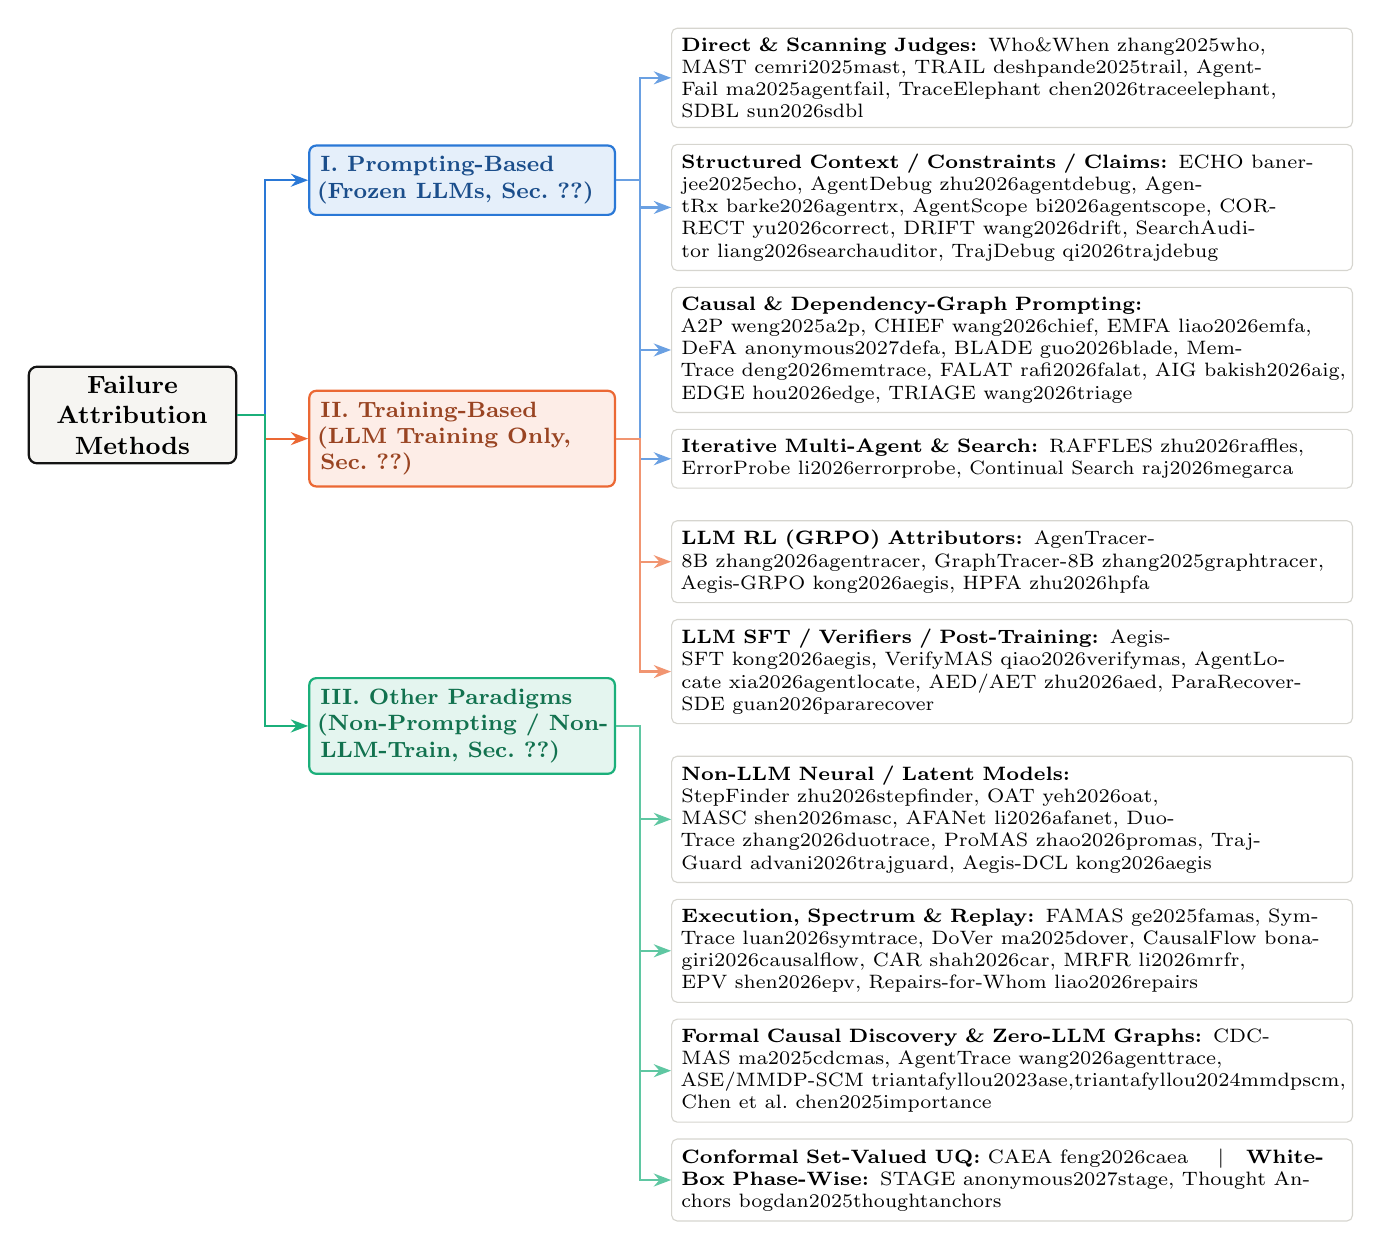
\begin{tikzpicture}[
  node distance=4mm and 7mm,
  root/.style={rectangle,rounded corners=3pt,draw=ink,fill=surface,thick,font=\small\bfseries,align=center,minimum height=11mm,text width=24mm},
  cat/.style={rectangle,rounded corners=2.5pt,thick,font=\footnotesize\bfseries,align=left,minimum height=8mm,text width=36mm,inner sep=4pt},
  sub/.style={rectangle,rounded corners=2pt,draw=rulec,fill=white,font=\scriptsize,align=left,text width=84mm,inner sep=3.5pt},
  edge/.style={-{Stealth[length=2.2mm]},thick,draw=ink3}
]
\node[root] (R) {Failure\\Attribution\\Methods};

% Category I
\node[cat,draw=s1,fill=s1!12,text=s1!65!black,above right=19mm and 9mm of R] (C1) {\textbf{I. Prompting-Based}\\(Frozen LLMs, Sec.~\ref{sec:prompting})};
\node[sub,right=7mm of C1,yshift=13mm] (C1a) {\textbf{Direct \& Scanning Judges:} Who\&When~\citep{zhang2025who}, MAST~\citep{cemri2025mast}, TRAIL~\citep{deshpande2025trail}, AgentFail~\citep{ma2025agentfail}, TraceElephant~\citep{chen2026traceelephant}, SDBL~\citep{sun2026sdbl}};
\node[sub,below=2mm of C1a] (C1b) {\textbf{Structured Context / Constraints / Claims:} ECHO~\citep{banerjee2025echo}, AgentDebug~\citep{zhu2026agentdebug}, AgentRx~\citep{barke2026agentrx}, AgentScope~\citep{bi2026agentscope}, CORRECT~\citep{yu2026correct}, DRIFT~\citep{wang2026drift}, SearchAuditor~\citep{liang2026searchauditor}, TrajDebug~\citep{qi2026trajdebug}};
\node[sub,below=2mm of C1b] (C1c) {\textbf{Causal \& Dependency-Graph Prompting:} A2P~\citep{weng2025a2p}, CHIEF~\citep{wang2026chief}, EMFA~\citep{liao2026emfa}, DeFA~\citep{anonymous2027defa}, BLADE~\citep{guo2026blade}, MemTrace~\citep{deng2026memtrace}, FALAT~\citep{rafi2026falat}, AIG~\citep{bakish2026aig}, EDGE~\citep{hou2026edge}, TRIAGE~\citep{wang2026triage}};
\node[sub,below=2mm of C1c] (C1d) {\textbf{Iterative Multi-Agent \& Search:} RAFFLES~\citep{zhu2026raffles}, ErrorProbe~\citep{li2026errorprobe}, Continual Search~\citep{raj2026megarca}};

% Category II
\node[cat,draw=s2,fill=s2!12,text=s2!65!black,right=9mm of R,yshift=-3mm] (C2) {\textbf{II. Training-Based}\\(LLM Training Only, Sec.~\ref{sec:training})};
\node[sub,below=4mm of C1d] (C2a) {\textbf{LLM RL (GRPO) Attributors:} AgenTracer-8B~\citep{zhang2026agentracer}, GraphTracer-8B~\citep{zhang2025graphtracer}, Aegis-GRPO~\citep{kong2026aegis}, HPFA~\citep{zhu2026hpfa}};
\node[sub,below=2mm of C2a] (C2b) {\textbf{LLM SFT / Verifiers / Post-Training:} Aegis-SFT~\citep{kong2026aegis}, VerifyMAS~\citep{qiao2026verifymas}, AgentLocate~\citep{xia2026agentlocate}, AED/AET~\citep{zhu2026aed}, ParaRecover-SDE~\citep{guan2026pararecover}};

% Category III
\node[cat,draw=s3,fill=s3!12,text=s3!65!black,below right=27mm and 9mm of R] (C3) {\textbf{III. Other Paradigms}\\(Non-Prompting / Non-LLM-Train, Sec.~\ref{sec:other})};
\node[sub,below=4mm of C2b] (C3a) {\textbf{Non-LLM Neural / Latent Models:} StepFinder~\citep{zhu2026stepfinder}, OAT~\citep{yeh2026oat}, MASC~\citep{shen2026masc}, AFANet~\citep{li2026afanet}, DuoTrace~\citep{zhang2026duotrace}, ProMAS~\citep{zhao2026promas}, TrajGuard~\citep{advani2026trajguard}, Aegis-DCL~\citep{kong2026aegis}};
\node[sub,below=2mm of C3a] (C3b) {\textbf{Execution, Spectrum \& Replay:} FAMAS~\citep{ge2025famas}, SymTrace~\citep{luan2026symtrace}, DoVer~\citep{ma2025dover}, CausalFlow~\citep{bonagiri2026causalflow}, CAR~\citep{shah2026car}, MRFR~\citep{li2026mrfr}, EPV~\citep{shen2026epv}, Repairs-for-Whom~\citep{liao2026repairs}};
\node[sub,below=2mm of C3b] (C3c) {\textbf{Formal Causal Discovery \& Zero-LLM Graphs:} CDC-MAS~\citep{ma2025cdcmas}, AgentTrace~\citep{wang2026agenttrace}, ASE/MMDP-SCM~\citep{triantafyllou2023ase,triantafyllou2024mmdpscm}, Chen et al.~\citep{chen2025importance}};
\node[sub,below=2mm of C3c] (C3d) {\textbf{Conformal Set-Valued UQ:} CAEA~\citep{feng2026caea} \quad\textbar\quad \textbf{White-Box Phase-Wise:} STAGE~\citep{anonymous2027stage}, Thought Anchors~\citep{bogdan2025thoughtanchors}};

% Edges
\draw[edge,draw=s1] (R.east) -- ++(3.5mm,0) |- (C1.west);
\draw[edge,draw=s2] (R.east) -- ++(3.5mm,0) |- (C2.west);
\draw[edge,draw=s3] (R.east) -- ++(3.5mm,0) |- (C3.west);

\foreach \n in {C1a,C1b,C1c,C1d} \draw[edge,draw=s1!70] (C1.east) -- ++(3mm,0) |- (\n.west);
\foreach \n in {C2a,C2b} \draw[edge,draw=s2!70] (C2.east) -- ++(3mm,0) |- (\n.west);
\foreach \n in {C3a,C3b,C3c,C3d} \draw[edge,draw=s3!70] (C3.east) -- ++(3mm,0) |- (\n.west);
\end{tikzpicture}%
}
\caption{Taxonomy of failure attribution methods for LLM agent systems, strictly separating prompting-based inference over frozen LLMs (Category~I), LLM parameter training (Category~II), and five alternative methodological paradigms (Category~III).}
\label{fig:taxonomy}
\end{figure}
\clearpage

% !TEX root = ../main.tex
\section{Landscape Overview and Comparative Benchmarks}\label{sec:overview}

Before examining each paradigm in detail, Table~\ref{tab:master} provides a unified side-by-side matrix of representative methods across all three categories, comparing their core attribution mechanism, supervision requirements, target granularity, online vs.\ offline timing, and whether they support downstream repair or rollback. Table~\ref{tab:whowhen} then compiles published benchmark performance on \textbf{Who\&When}~\citep{zhang2025who}---the de facto common testbed across paradigms---while explicitly surfacing backbone and ground-truth (\code{w/ G} vs.\ \code{w/o G}) differences.

\begin{center}
\scriptsize
\setlength{\tabcolsep}{3.5pt}
\begin{longtable}{@{}>{\RaggedRight\bfseries}p{2.55cm}>{\RaggedRight}p{1.55cm}>{\RaggedRight}p{4.4cm}>{\RaggedRight}p{2.45cm}>{\RaggedRight}p{2.1cm}p{0.8cm}p{0.65cm}@{}}
\caption{Master taxonomy of failure attribution methods across Prompting-Based (I), LLM Training-Based (II), and Other Paradigms (III). \emph{Timing}: Off = post-hoc offline, On = online/real-time. \emph{Rep}: \yes{} = explicitly evaluated on downstream repair/rollback, \no{} = localization only. \webtag{} marks papers identified via extended literature search beyond \code{papers/methods/}.}\label{tab:master}\\
\toprule
Method & Venue/Yr & Core Mechanism & Supervision & Granularity & Time & Rep \\
\midrule
\endfirsthead
\toprule
Method & Venue/Yr & Core Mechanism & Supervision & Granularity & Time & Rep \\
\midrule
\endhead
\midrule
\multicolumn{7}{r}{\scriptsize\itshape Continued on next page}\\
\endfoot
\bottomrule
\endlastfoot

% --- Category I ---
\multicolumn{7}{@{}l}{\textbf{\color{s1!70!black}Category I: Prompting-Based Methods (Frozen LLMs)}}\\
\midrule
Who\&When~\citep{zhang2025who} & ICML'25 & All-at-Once, Step-by-Step, Binary Search judges & Zero-shot & Agent + Step & Off & \no \\
MAST~\citep{cemri2025mast} & NeurIPS'25 & 14-mode grounded taxonomy + calibrated o1 judge & Taxonomy prompt & Mode (trace) & Off & \yes \\
TRAIL~\citep{deshpande2025trail} & arXiv'25 & OpenTelemetry span-level judge + 3-way taxonomy & Taxonomy prompt & Span + Mode & Off & \no \\
AgentFail~\citep{ma2025agentfail} & arXiv'25 & Taxonomy-guided scanning for workflow platforms & Taxonomy prompt & Node + Mode & Off & \no \\
SDBL~\citep{sun2026sdbl}\,\webtag & AAAI'26 & Scope delineation (narrowing) $\to$ fine localization & Zero-shot & Agent + Step & Off & \no \\
ECHO~\citep{banerjee2025echo} & NeurIPS'25 & 4-layer regex hierarchy ($L_1$--$L_4$) + 6-persona voting & Zero-shot & Agent + Step & Off & \no \\
AgentDebug~\citep{zhu2026agentdebug} & ICML'26 & 4-module taxonomy scan $\to$ critical step $\to$ feedback & Taxonomy prompt & Step + Mod + Mode & Off & \yes \\
AgentRx~\citep{barke2026agentrx} & EMNLP'26F & Synthesize guarded constraints $\to$ violation log $\to$ judge & Policy / schema & Step + Mode (9) & Off & \no \\
AgentScope~\citep{bi2026agentscope} & arXiv'26 & Neuro-symbolic ReAG graph + neural invariants & Invariant specs & Step + Mode (10) & Off & \no \\
CORRECT~\citep{yu2026correct} & ICML'26 & Online cache of distilled error schemata $\langle\Sigma,C,H\rangle$ & Seed error logs & Agent + Step & Both & \no \\
DRIFT~\citep{wang2026drift} & arXiv'26 & Claim Keeper $\to$ Support Seeker $\to$ Dependency Tracer & Zero-shot & Error spans & Off & \no \\
SearchAuditor~\citep{liang2026searchauditor} & arXiv'26 & 3 parallel audit branches + grounded adjudication & Zero-shot & Step + Mode + Fix & Off & \yes \\
TrajDebug~\citep{qi2026trajdebug}\,\webtag & EMNLP'26F & Multi-granularity compression + error-lifecycle tracking & Zero-shot & Step + Lifecycle & Off & \yes \\
A2P~\citep{weng2025a2p} & arXiv'25 & Single-pass Abduct--Act--Predict causal scaffolding & Zero-shot & Agent + Step & Off & \no \\
CHIEF~\citep{wang2026chief} & arXiv'26 & RAG Hierarchical Causal Graph $\to$ oracle backtrack $\to$ CF & RAG exemplars & Agent + Step & Off & \no \\
EMFA~\citep{liao2026emfa} & arXiv'26 & Symptom anchor + cascade/loop dual-branch + CF check & Zero-shot & Agent + Step & Off & \no \\
DeFA~\citep{anonymous2027defa} & ICLR'27sub & Protocol+semantic EDG $\to$ segmented FPG $\to$ adjudicator & Zero-shot & Agent + Step + Mode & Off & \yes \\
BLADE~\citep{guo2026blade} & arXiv'26 & Probabilistic Jev dep.\ graph $\to$ handoff contract audit & Zero-shot & Agent + Step & Off & \no \\
MemTrace~\citep{deng2026memtrace} & arXiv'26 & Instrumented memory var--op graph + graph/regex agent & Code instrum. & Operation + Mode & Off & \yes \\
FALAT~\citep{rafi2026falat}\,\webtag & arXiv'26 & Task prior + typed dep.\ pruning + CF sufficiency & Zero-shot & Agent + Step & Off & \no \\
AIG~\citep{bakish2026aig}\,\webtag & arXiv'26 & Adaptive influence graph + agent-directed traversal & Zero-shot & Agent + Step & Off & \no \\
EDGE~\citep{hou2026edge}\,\webtag & EMNLP'26F & CF-validated Error Dependency Graph $\to$ 2-stage judge & CF rollouts & Multi-error modes & Off & \yes \\
RAFFLES~\citep{zhu2026raffles} & UIST'26 & Central Judge + Evaluator critiques in iterative loop & Zero-shot & Agent + Step & Off & \no \\
ErrorProbe~\citep{li2026errorprobe} & ACL'26F & MAST cues + backward trace + 3-agent team + verified mem. & Exec.\ feedback & Agent + Step & Off & \no \\
MegaRCA~\citep{raj2026megarca}\,\webtag & arXiv'26 & Continual iterative search nudging unexamined evidence & Zero-shot & Step + Mode & Off & \no \\
\midrule
% --- Category II ---
\multicolumn{7}{@{}l}{\textbf{\color{s2!70!black}Category II: Training-Based Methods (LLM Training Only)}}\\
\midrule
AgenTracer~\citep{zhang2026agentracer} & ICLR'26 & KL-free GRPO on Qwen3-8B; Gaussian step + agent reward & CF replay + FI & Agent + Step & Off & \yes \\
GraphTracer~\citep{zhang2025graphtracer} & arXiv'25 & RL on Qwen3-8B over IDGs; source + GED path reward & IDG-aware FI & Node + Path & Off & \yes \\
Aegis-SFT/GRPO~\citep{kong2026aegis} & ICLR'26 & SFT \& GRPO (Qwen2.5/3) w/ partial-credit pair rewards & Adaptive FI (9.5k) & Agent + Mode(s) & Off & \no \\
HPFA~\citep{zhu2026hpfa} & COLM'26 & Paired hypergraph data $\to$ SFT + on-policy rollout GRPO & Success/fail pairs & Step + Type + Desc & Off & \yes \\
VerifyMAS~\citep{qiao2026verifymas}\,\webtag & NeurIPS'26 & Error-first hypothesis verification via SFT LLM verifier & Taxonomy hyp.\ data & Mode + Agent & Off & \no \\
AgentLocate~\citep{xia2026agentlocate}\,\webtag & COLM'26 & Multi-perspective verification + lightweight LLM SFT & Annotated traces & Agent + Step & Off & \no \\
AED / AET~\citep{zhu2026aed}\,\webtag & arXiv'26 & 50k replay-verified error--diagnosis pairs for SFT/DPO & Replay-verified & Step + Diag + Fix & Off & \yes \\
\midrule
% --- Category III ---
\multicolumn{7}{@{}l}{\textbf{\color{s3!65!black}Category III: Other Paradigms (Non-Prompting \& Non-LLM-Training)}}\\
\midrule
StepFinder~\citep{zhu2026stepfinder} & KDD'26 & Frozen Qwen3 embeds $\to$ BiLSTM + agent-aware attn & Labeled fail logs & Step (ranked) & Off & \no \\
OAT~\citep{yeh2026oat} & NeurIPS'26 & One-class Neural CDE on frozen LLM hidden states & Success logs only & Error step set & Off & \no \\
MASC~\citep{shen2026masc} & arXiv'26 & Frozen LLM + trainable head + normal prototype prior & Normal logs only & Step (online) & On & \yes \\
AFANet~\citep{li2026afanet}\,\webtag & arXiv'26 & Lightweight GNN over semantic-structural trace graphs & Labeled fail logs & Agent + Mode & Off & \no \\
DuoTrace~\citep{zhang2026duotrace}\,\webtag & arXiv'26 & VAE + Tree-LSTM anomaly pre-filter before attribution & Normal + replay & Agent + Step & Off & \no \\
ProMAS~\citep{zhao2026promas}\,\webtag & arXiv'26 & Causal Delta Features $\to$ quantized Vector Markov Space & Normal/fail logs & Step forecast & On & \no \\
Aegis-DCL~\citep{kong2026aegis} & ICLR'26 & Text encoder + MIL attention + agent/error prototypes & Paired pos/neg & Agent + Mode(s) & Off & \no \\
FAMAS~\citep{ge2025famas} & arXiv'25 & Repeated replay + hierarchical clustering + MAS SBFL & Env.\ replay & Agent + Action & Off & \no \\
SymTrace~\citep{luan2026symtrace} & arXiv'26 & Deterministic prefix-hash replay + suspicious-node fix & Env.\ replay & Actionable node & Off & \yes \\
DoVer~\citep{ma2025dover}\,\webtag & arXiv'25 & Active message/plan interventions + outcome replay & Env.\ replay & Agent + Step & Off & \yes \\
CausalFlow~\citep{bonagiri2026causalflow}\,\webtag & arXiv'26 & Step-level interventions $\to$ Causal Resp.\ Scores (CRS) & Env.\ replay & Step + Min.\ fix & Off & \yes \\
CAR / MRFR~\citep{shah2026car,li2026mrfr}\,\webtag & arXiv'26 & SCM $\text{do}(\cdot)$ replay / Graph-Constrained Joint Replay & Env.\ replay & Step / Repair set & Off & \yes \\
EPV~\citep{shen2026epv}\,\webtag & arXiv'26 & Monte Carlo prefix value $V(h_t)$ to certify PNR & Env.\ replay & PNR step & Off & \no \\
CDC-MAS~\citep{ma2025cdcmas}\,\webtag & arXiv'25 & Causal inversion + Shapley values + causal discovery & Execution logs & Agent + Step & Off & \yes \\
AgentTrace~\citep{wang2026agenttrace}\,\webtag & arXiv'26 & Zero-LLM causal graph backward traversal + ranking & Execution logs & Root-cause step & Off & \no \\
CAEA~\citep{feng2026caea} & arXiv'26 & Sequential filtration CP (LF/RF/TWF) + rollback sets & Calib.\ set ($n$) & Contiguous set & Off & \yes \\
STAGE~\citep{anonymous2027stage} & ICLR'27sub & White-box VLA stage readers + entropy decomposition & Episode fail label & Phase (A/R/D) & On & \no \\
\end{longtable}
\end{center}

\begin{table}[h!]
\centering\footnotesize
\caption{Reported top-1 accuracy (\%) on \textbf{Who\&When}~\citep{zhang2025who} (Hand-Crafted: $58$ logs; Algorithm-Generated: $126$ logs) compiled from original papers. \textbf{Caution:} methods use different base LLMs, prompt interfaces, and ground-truth access (\code{w/ G} = task answer given; \code{w/o G} = trajectory only), so rows are not strictly apples-to-apples.}
\label{tab:whowhen}
\fitbox{\begin{tabular}{@{}l l l c c c c@{}}
\toprule
& & & \multicolumn{2}{c}{\textbf{Hand-Crafted (HC)}} & \multicolumn{2}{c}{\textbf{Algorithm-Generated (AG)}} \\
\cmidrule(lr){4-5}\cmidrule(lr){6-7}
Method & Category & Backbone / Setup & Agent (\%) & Step (\%) & Agent (\%) & Step (\%) \\
\midrule
Random~\citep{zhang2025who} & Baseline & Uniform heuristic & 12.00 & 4.20 & 29.10 & 19.10 \\
All-at-Once~\citep{zhang2025who,wang2026chief} & I (Prompt) & GPT-4o (w/ G $\mid$ w/o G) & 50.00 $\mid$ 48.28 & 5.17 $\mid$ 5.17 & 54.33 $\mid$ 59.52 & 12.50 $\mid$ 15.87 \\
Step-by-Step~\citep{zhang2025who,liao2026emfa} & I (Prompt) & GPT-4o (w/ G $\mid$ w/o G) & 36.00 $\mid$ 34.30 & 6.90 $\mid$ 6.90 & 35.20 $\mid$ 28.30 & 25.51 $\mid$ 17.80 \\
Binary Search~\citep{zhang2025who,liao2026emfa} & I (Prompt) & GPT-4o (w/ G $\mid$ w/o G) & 51.70 $\mid$ 36.20 & 6.90 $\mid$ 6.90 & 44.13 $\mid$ 30.10 & 23.98 $\mid$ 16.60 \\
A2P~\citep{weng2025a2p} & I (Prompt) & Single-pass causal scaffold & 58.62 & 29.31 & 65.40 & 47.46 \\
ECHO~\citep{banerjee2025echo} & I (Prompt) & Claude-3.5-Sonnet (w/ G $\mid$ w/o G) & 68.40 $\mid$ 67.90 & 28.10 $\mid$ 26.80 & 68.80 $\mid$ 67.20 & 28.80 $\mid$ 27.20 \\
RAFFLES~\citep{zhu2026raffles} & I (Prompt) & Claude-Sonnet-4 (Table~1 / Intro) & --- & 20.69 / 27.59 & --- & 51.59 \\
SDBL~\citep{sun2026sdbl,liao2026emfa} & I (Prompt) & Two-stage scope (w/o G) & 68.52 & 27.78 & 63.49 & 39.68 \\
CHIEF~\citep{wang2026chief} & I (Prompt) & DeepSeek-V3.2 think (w/ G $\mid$ w/o G) & \textbf{77.59} $\mid$ 72.41 & 29.31 $\mid$ 29.31 & \textbf{76.80} $\mid$ 68.80 & \textbf{52.00} $\mid$ 45.60 \\
FALAT~\citep{rafi2026falat,liao2026emfa} & I (Prompt) & Dep.-guided search (w/o G) & 73.00 & 29.10 & 59.70 & 38.00 \\
EMFA~\citep{liao2026emfa} & I (Prompt) & GPT-4o (w/o G) & 74.14 & 32.76 & 66.67 & 50.00 \\
BLADE~\citep{guo2026blade} & I (Prompt) & Jev interface (w/o G) & 58.60 & 31.00 & 66.70 & \textbf{54.00} \\
DeFA~\citep{anonymous2027defa} & I (Prompt) & GLM-5.2 (w/o G, \emph{combined} 184) & \multicolumn{4}{c}{Combined HC+AG: Agent \textbf{72.3\%}, Step \textbf{52.7\%} (Step$\pm$1: 57.1\%)} \\
\midrule
AgenTracer-8B~\citep{zhang2026agentracer} & II (LLM RL) & Qwen3-8B GRPO (w/ G $\mid$ w/o G) & 69.10 $\mid$ 63.82 & 20.68 $\mid$ 20.68 & 69.62 $\mid$ 63.73 & 42.86 $\mid$ 37.30 \\
GraphTracer-8B~\citep{zhang2025graphtracer} & II (LLM RL) & Qwen3-8B IDG-RL (w/ G $\mid$ w/o G) & 74.91 $\mid$ 69.74 & 28.63 $\mid$ 27.97 & 76.64 $\mid$ 67.42 & 49.97 $\mid$ 44.35 \\
\midrule
StepFinder~\citep{zhu2026stepfinder} & III (Non-LLM) & Qwen3-Emb + BiLSTM+Attn (w/o G) & --- & 22.99 & --- & 29.63 \\
FAMAS~\citep{ge2025famas} & III (Spectrum) & Qwen2.5-72B replay + SBFL (w/ G) & 62.07 & \textbf{41.38} & 55.56 & 23.81 \\
\bottomrule
\end{tabular}}
\end{table}

Two macro-patterns immediately stand out from Table~\ref{tab:whowhen}. First, \textbf{step-level localization remains dramatically harder than agent-level attribution}: even strong graph-guided prompting methods exceeding $70\%$ agent accuracy typically achieve $29\%$--$33\%$ exact step accuracy on the longer, realistic Hand-Crafted subset. Second, \textbf{structured prompting over frontier models has largely caught up to or surpassed first-generation 8B RL-trained tracers on Who\&When}, yet at $2.5\times$--$10\times$ higher inference token cost and latency---whereas lightweight non-LLM models (StepFinder, OAT, MASC, AFANet) trade peak exact-step accuracy for $5\times$--$5000\times$ speedups and online deployability.

% !TEX root = ../main.tex
\section{Category I: Prompting-Based Methods}\label{sec:prompting}

\begin{summarybox}[s1]{Paradigm Summary \hfill \promptbadge}
Prompting-based methods keep all LLM weights \textbf{frozen} and perform failure attribution purely through inference-time scaffolding: log partitioning, failure taxonomies, programmatic/semantic constraint checking, dependency and causal graph construction, or iterative multi-agent adjudication. They require \emph{no model training} and immediately inherit gains from stronger foundation models, but face fundamental tensions between context length, inference token cost, and vulnerability to late-stage symptom bias.
\end{summarybox}

Across the literature, prompting-based attribution has rapidly progressed through four increasingly structured architectural waves.

\subsection{Direct and Sequential Log-Scanning Judges}
The earliest wave feeds raw or minimally segmented execution logs directly to an LLM judge.

\paragraph{Who\&When Baselines~\citep{zhang2025who}}
Formulating automated MAS failure attribution alongside the $184$-trace Who\&When benchmark ($126$ CaptainAgent Algorithm-Generated and $58$ Magentic-One Hand-Crafted logs), Zhang et al.\ establish three canonical prompting protocols:
(i)~\textbf{All-at-Once}, which feeds the entire trajectory in a single prompt to predict $(i^*, t^*)$---giving global visibility at low call count ($O(1)$) but suffering severe long-context dilution;
(ii)~\textbf{Step-by-Step}, which incrementally reveals prefixes $\tau_{\le t}$ and halts at the first detected mistake---sharpening local focus at $O(T)$ cost but lacking downstream outcome awareness; and
(iii)~\textbf{Binary Search}, which recursively halves the trace in $O(\log T)$ calls---improving scalability but failing when deciding which half contains a subtle upstream root cause. Even frontier reasoning models (o1, DeepSeek-R1) achieved at most $53.5\%$ agent accuracy and $14.2\%$ step accuracy, collapsing near $0\%$ on the longest logs.

\paragraph{Taxonomy-Guided Judges: MAST~\citep{cemri2025mast}, TRAIL~\citep{deshpande2025trail}, and AgentFail~\citep{ma2025agentfail}}
Several foundational works pair raw log judging with empirically grounded failure taxonomies. \textbf{MAST} derives $14$ failure modes across $3$ categories (System Design, Inter-Agent Misalignment, Task Verification; human $\kappa=0.88$) from $1{,}642$ traces and builds a calibrated OpenAI o1 LLM-as-a-Judge pipeline ($\kappa=0.77$--$0.79$ with humans). \textbf{TRAIL} targets OpenTelemetry-formatted single- and multi-agent traces ($148$ traces, $841$ span-level errors across Reasoning, Execution, and Planning), showing that even Gemini-2.5-Pro scores only $11\%$ joint localization--classification accuracy. \textbf{AgentFail} studies $307$ failure logs from low-code workflow platforms (Dify, Coze, n8n, AutoGen), demonstrating that injecting its platform/workflow/agent taxonomy into All-at-Once, Step-by-Step, and Binary Search boosts root-cause accuracy by $15$--$20$ percentage points (from $8.3\%$--$13.0\%$ to $24.1\%$--$33.6\%$), yet leaving two-thirds of cases unsolved.

\paragraph{Full-Observability Auditing and Two-Stage Scoping: TraceElephant~\citep{chen2026traceelephant} and SDBL~\citep{sun2026sdbl}\,\webtag}
\textbf{TraceElephant} ($220$ fully observable, reproducible traces across CaptainAgent, Magentic-One, and mini-SWE-agent) reveals that supplying full step inputs, agent prompts, and architecture specs instead of output-only logs lifts LLM attribution accuracy by up to $76\%$, and that an agentic tool-equipped inspector outperforms static scanning. \textbf{SDBL} (\emph{Scope Delineation Before Localization}, AAAI 2026) directly addresses context overload by decoupling attribution into two prompting stages: first narrowing a long trajectory to a compact suspicious candidate window (via stepwise or expertise-assisted scoping), then performing fine-grained localization only inside the scoped subset ($68.5\%$ HC / $63.5\%$ AG agent; $27.8\%$ HC / $39.7\%$ AG step on Who\&When w/o G).

\subsection{Structured Context, Constraint, Schema, and Claim-Auditing Pipelines}
To overcome brittle raw-text judging, a second wave transforms traces into structured intermediate artifacts---compressed hierarchies, modular checks, explicit constraints, cached error schemata, or claim ledgers---before final adjudication.

\paragraph{ECHO~\citep{banerjee2025echo}}
ECHO (\emph{Error attribution through Contextual Hierarchy and Objective consensus}) tackles long-context degradation via three decoupled mechanisms: (1) a \textbf{four-layer regex-based hierarchical context} around each target step---$L_1$ immediate neighbors ($\tau_{i\pm 1}$, verbatim), $L_2$ local ($\tau_{i\pm 2,3}$, conclusions/transitions), $L_3$ distant ($\tau_{i\pm 4..6}$, state/error summaries), and $L_4$ global milestones; (2) a \textbf{panel of 6 specialized analyst personas} (Conservative, Liberal, Detail-Focused, Pattern-Focused, Skeptical, General; $3$ sampled per trace at temperatures $0.3$--$0.9$) outputting step likelihoods and alternative hypotheses; and (3) \textbf{confidence-weighted consensus voting} ($\delta=0.3$). With Claude-3.5-Sonnet, ECHO reaches $68.4\%$ HC / $68.8\%$ AG agent accuracy and $28.1\%$ HC / $28.8\%$ AG step accuracy on Who\&When; switching regex compression to LLM extraction raises HC step accuracy to $43.8\%$ but triples token cost ($166\text{K}$ vs.\ $54\text{K}$ tokens).

\paragraph{AgentDebug~\citep{zhu2026agentdebug}}
Targeting single-agent rollouts decomposed into four cognitive modules (\emph{Memory, Reflection, Planning, Action}) on AgentErrorBench (ALFWorld, GAIA, WebShop), AgentDebug executes a three-stage prompting loop: (1) fine-grained per-step, per-module mapping onto the modular \emph{AgentErrorTaxonomy}; (2) LLM critical-error detection selecting the earliest root-cause step $t^*$; and (3) iterative re-rollout from $t^*$ with targeted corrective feedback. On AgentErrorBench with GPT-4.1, AgentDebug achieves $42\%$ step accuracy and $32\%$ strict all-correct accuracy ($+17\%$ step and $+24\%$ all-correct over baselines), driving up to $+26\%$ relative downstream task recovery.

\paragraph{AgentRx~\citep{barke2026agentrx}}
Inspired by software design-by-contract, AgentRx diagnoses the \emph{first unrecoverable failure} across API workflows ($\tau$-bench), incident management (Flash), and web/file MAS (Magentic-One). Given domain policies and tool schemas, AgentRx automatically synthesizes both \textbf{programmatic constraints} and \textbf{semantic natural-language guarded constraints}, evaluates each constraint step-by-step to produce an auditable \textbf{validation log} $\mathcal{V} = \{(k, C, e)\}$ of violations with grounded evidence, and feeds $\mathcal{V}$ plus a grounded-theory $9$-category checklist to an LLM judge. Across the three domains (using GPT-5), AgentRx delivers $+23.6\%$ absolute step-localization and $+22.9\%$ failure-category improvements over direct baselines.

\paragraph{AgentScope~\citep{bi2026agentscope}}
AgentScope advances a \textbf{neuro-symbolic} diagnostic pipeline: (1) instrumentation and selective LLM parsing convert raw traces into a \textbf{Reasoning-Action Graph (ReAG)} with aligned semantic fields (role, step purpose, actions, missing-info signals); (2) a library of \textbf{neural invariants}---formal failure-mode predicates backed by targeted JSON-returning LLM functions spanning $10$ failure types across Reasoning, Control-flow, and Action---scans the ReAG to retain multiple evidence-backed candidate hypotheses; and (3) a decisive-error judge selects the single fault whose downstream impact best explains task failure. AgentScope achieves $25.4\%$--$77.8\%$ step accuracy on Who\&When-AG, $22.4\%$--$34.5\%$ on HC, and $28.4\%$--$54.1\%$ on the newly introduced $303$-trace AgentErrata benchmark.

\paragraph{CORRECT~\citep{yu2026correct}}
Observing that $>80\%$ of failed Who\&When traces exhibit pairwise BERT cosine similarity $>0.8$ yet naive few-shot ICL degrades accuracy due to $32\text{K}+$ context bloat, CORRECT introduces a training-free \textbf{online error-schema cache}. From seed annotated failures, an LLM distills compact structured schemata $S = \langle \Sigma, C, H \rangle$ containing \emph{Error Signatures} $\Sigma$, \emph{Error Context Analysis} $C$, and actionable \emph{Detection Heuristics} $H$. At inference, semantically relevant schemata are retrieved in sub-seconds to guide targeted localization, yielding up to $+19.8\%$ accuracy gains on Who\&When and $+28.7\%$ average gains across seven MAS applications on CORRECT-Error ($2{,}000+$ traces) with zero LLM retraining.

\paragraph{Domain-Specialized Auditing: DRIFT~\citep{wang2026drift}, SearchAuditor~\citep{liang2026searchauditor}, and TrajDebug~\citep{qi2026trajdebug}\,\webtag}
Long-horizon search and deep-research agents rarely crash with exceptions; instead, they commit early to unsupported facts that look fluent downstream.
\textbf{DRIFT} reframes span-level localization (on its $1{,}000$-instance TELBench) around \textbf{claim-centric auditing}: (A)~\emph{Claim Keeper} builds a global claim ledger $\mathcal{L} = \{(a_k, i_k, b_k, U_k, \tau_k, \sigma_k)\}$ separating benign exploratory queries from settled commitments; (B)~\emph{Support Seeker} verifies trajectory evidence (\code{DIRECT/WEAK/...}); and (C)~\emph{Dependency Tracer} propagates unsupported commitments forward/backward to flag consequential error spans, boosting F1 and first-error accuracy by up to $+30$~pp.
\textbf{SearchAuditor} (on SearchAuditBench: $1{,}243$ trajectories averaging $73.1$ messages / $65.1\text{K}$ tokens) runs \textbf{three complementary parallel audit branches}, adjudicates their findings over a compact evidence-grounded trajectory view, and synthesizes rubric-graded repair directives---lifting GPT-5.5 end-to-end pass rate from $26.6\%$ to $32.3\%$ and fixing $17.4\%$ of Kimi-K2.6's live failures on LiveBrowseComp.
\textbf{TrajDebug}~\citep{qi2026trajdebug} combines multi-granularity history compression with \textbf{error-lifecycle state tracking}, explicitly distinguishing local errors that were subsequently resolved from persistent faults that drove final failure.

\subsection{Causal-Reasoning, Dependency-Graph, and Propagation-Guided Prompting}
A third---and currently highest-performing---prompting wave moves beyond flat logs and independent step checks by prompting LLMs to reconstruct explicit \textbf{causal, information-dependency, or error-propagation graphs} and verify counterfactual decisiveness.

\paragraph{A2P Scaffolding~\citep{weng2025a2p}}
A2P (\emph{Abduct--Act--Predict}, co-authored by DeepScientist) bridges the counterfactual inference gap within a \emph{single} LLM pass by imposing Pearl's three-step causal ladder alongside explicit contextual step numbering: (1)~\textbf{Abduction} infers latent root causes (assumptions, knowledge gaps) behind observed actions; (2)~\textbf{Action} specifies a minimal corrective intervention; and (3)~\textbf{Prediction} mentally simulates the post-intervention trajectory to verify task resolution. On Who\&When, A2P boosts step accuracy $2.85\times$ on AG ($47.46\%$) and $2.43\times$ on HC ($29.31\%$) with only $\sim 25\%$ latency overhead; ablations reveal that explicit step numbering alone accounts for $+29.7$~pp.

\paragraph{CHIEF~\citep{wang2026chief}}
CHIEF transforms flat logs into a two-level \textbf{Hierarchical Causal Graph (HCG)} $G=(V_{\text{sub}}\cup V_{\text{agt}}, E)$ in three phases: (1)~RAG-guided task decomposition (retrieving exemplar plans from GAIA/AssistantBench) refined by trajectory-aligned reflection yields contiguous subtask nodes and intra-subtask agent DAGs; (2)~\textbf{Hierarchical Oracle-Guided Backtracking} synthesizes virtual oracles to prune irrelevant subtasks top-down; and (3)~\textbf{Progressive Counterfactual Causal Screening} tests four counterfactual patterns (local, planning-control, data-flow, deviation-aware) to separate root causes from propagated symptoms. With DeepSeek-V3.2 (thinking), CHIEF attains $77.6\%/72.4\%$ HC and $76.8\%/68.8\%$ AG agent accuracy, and $29.3\%$ HC / $52.0\%/45.6\%$ AG step accuracy (w/ G $\mid$ w/o G) at $2.5$--$3\times$ All-at-Once token cost ($6$--$8\times$ cheaper than replay-based FAMAS).

\paragraph{EMFA~\citep{liao2026emfa}}
Noting that prior graph methods miss persistent unresolved interaction loops, EMFA (\emph{Error-Propagation Modeling for Failure Attribution}) executes five stages without requiring task ground truth: (1)~extracts a query-only success specification $C_{\text{success}}$ to anchor the terminal failure symptom $x_{\text{final}}$; (2)~constructs a two-level step/subtask dependency structure $\mathcal{H}$; (3)~explicitly models both \textbf{cascading propagation chains} and \textbf{persistent interaction loops}; (4)~\textbf{dual-branch candidate screening} extracts top candidates from both branches; and (5)~\textbf{counterfactual decisive-error verification} selects $(a^*, i^*)$. With GPT-4o (w/o G), EMFA sets strong step accuracy on Who\&When: $32.76\%$ HC ($+3.45$~pp over CHIEF) and $50.00\%$ AG ($+4.40$~pp), with $74.14\%$ HC agent accuracy.

\paragraph{DeFA~\citep{anonymous2027defa}}
DeFA (\emph{Dependency-Guided Failure Attribution}) decouples \textbf{protocol relations} (framework-induced conventions such as delegation or tool-call/return pairs) from \textbf{semantic dependencies} (implicit cross-step content reuse) to build an \textbf{Event Dependency Graph (EDG)}. To scale to long and multimodal (image/video) traces, DeFA partitions trajectories into segments, supplying each segment with full local detail plus chronological summaries of all other segments for candidate event recall. It then constructs a \textbf{Failure Propagation Graph (FPG)} tracing upstream sources and downstream amplification/repair, before an LLM adjudicator selects $(t^*, a^*, y^*)$. On Who\&When (combined $184$ traces, w/o G), DeFA reaches $72.3\%$ agent and $52.7\%$ exact step accuracy with GLM-5.2 ($80.3\%$ step on Who\&When Pro text), and feeding DeFA diagnoses into Trace2Skill yields $+6$--$15$~pp downstream task gains.

\paragraph{BLADE~\citep{guo2026blade}}
BLADE (\emph{Blame Localization via Audited Dependency Evidence}) makes a sharp conceptual distinction: \emph{tracing where information came from is not the same as auditing how it was used}. Using the structured probabilistic judgment interface Jev, BLADE (1)~computes probabilities over four directed relations (\code{depends\_on}, \code{repeats}, \code{contradicts}, \code{repairs}) and retains edges $\ge \theta=0.3$; (2)~plans selective \textbf{contract auditing} over only the top-$K=2$ highest-probability sources per event ($13\%$--$23\%$ of all pairs), checking whether each receiving decision faithfully respected its source and task requirement spans (\emph{error introduction vs.\ propagation vs.\ repair}); and (3)~performs \textbf{defeasible global diagnosis} over the full blame graph. Across $1{,}228$ trajectories spanning five Who\&When and Who\&When Pro subsets (w/o G), BLADE beats All-at-Once by $2.2$--$11.1$~pp (macro average $66.8\%$ agent, $57.6\%$ step; $54.0\%$ Who\&When-AG step).

\paragraph{Stateful Memory and Emerging Graph-Prompting Works}
\textbf{MemTrace}~\citep{deng2026memtrace} extends dependency-graph attribution to stateful non-parametric memory systems (RAG, Mem0, EverMemOS) by instrumenting source code to emit a bipartite variable--operation execution graph $G=(V,O,E)$, then diagnosing extraction, update, retrieval, deletion, and response errors via graph-walking or regex-based operation search (\code{MemTrace-OBS})---enabling closed-loop prompt optimization ($+7.62$~pp end-task accuracy).
Recent web-sourced methods reinforce this graph-guided trend:
\textbf{FALAT}~\citep{rafi2026falat}\,\webtag frames attribution as hierarchical dependency-guided search using task-conditioned priors, typed dependencies to prune downstream carriers, and counterfactual sufficiency checks ($73.0\%$ HC agent, $29.1\%$ HC / $38.0\%$ AG step);
\textbf{Adaptive Influence Graphs (AIG)}~\citep{bakish2026aig}\,\webtag dynamically defines trace-specific node boundaries and non-adjacent inheritance edges for agent-directed traversal;
\textbf{EDGE}~\citep{hou2026edge}\,\webtag targets \emph{multi-error} attribution on TRAIL and MAST by validating an Error Dependency Graph via counterfactual rollouts to steer a two-stage LLM detector;
\textbf{TRIAGE}~\citep{wang2026triage}\,\webtag ranks candidate steps by severity and structural impact; and
\textbf{CockpitHAT}~\citep{wang2026cockpithat}\,\webtag applies dependency-graph hierarchical attribution to embodied multi-agent cockpits.

\subsection{Iterative Multi-Agent Adjudication and Continual Search}
Rather than relying on a fixed single-pass graph or static prompt pipeline, a fourth prompting family treats debugging as an \textbf{iterative, tool-using investigation} by specialized diagnostic agents.

\paragraph{RAFFLES~\citep{zhu2026raffles}}
RAFFLES formalizes the distinction between \emph{trivial} and \emph{critical} step faults and introduces an iterative \textbf{Judge--Evaluator} architecture: a central Judge proposes candidate faults and rationales, while a panel of specialized Evaluators independently critiques both the fault selection and the Judge's reasoning with natural-language confidence scores; the Judge reflects on these critiques over $K$ refinement iterations. On Who\&When with Claude-Sonnet-4, RAFFLES achieves $51.59\%$ step accuracy on AG and $20.69\%$--$27.59\%$ on HC, while exceeding $83\%$ on mathematical reasoning (ReasonEval).

\paragraph{ErrorProbe~\citep{li2026errorprobe}}
ErrorProbe combines taxonomy cues, backward tracing, multi-agent tool-grounded verification, and self-improving memory without updating LLM weights: (1)~a lightweight MAST detector tags local anomalies as heuristic priors; (2)~symptom-driven backward tracing prunes long histories to causally relevant turns; (3)~a three-agent diagnostic team (\textbf{Strategist, Investigator, Arbiter}) validates hypotheses using executable tools (e.g., code sandboxes); and (4)~a \textbf{verified-before-write episodic memory} commits reusable error/patch patterns \emph{only} when confirmed by executable evidence, preventing memory drift and enabling zero-training cross-domain transfer (e.g., KodCode $\to$ TracerTraj, reaching $73.2\%$ agent / $39.4\%$ step on TracerTraj and $60.3\%$ agent on Who\&When-Algo with Claude-3.7-Sonnet).

\paragraph{Continual Search (MegaRCA)~\citep{raj2026megarca}\,\webtag}
Arguing that one-shot LLM judges lock prematurely onto salient late symptoms in massive logs, Raj et al.\ cast long-horizon root-cause attribution as an iterative \textbf{search problem}, introducing Continual Search to repeatedly nudge diagnostic models toward unexamined evidence regions across long trajectories.

% !TEX root = ../main.tex
\section{Category II: Training-Based Methods (LLM Training Only)}\label{sec:training}

\begin{summarybox}[s2]{Paradigm Summary \hfill \trainbadge}
This category is restricted strictly to methods that \textbf{update LLM parameters} (via SFT, reinforcement learning such as GRPO, or preference optimization) to train specialized LLM failure attributors or verifiers. Methods that train non-LLM models (e.g., BiLSTMs, GNNs, Neural CDEs, VAEs, or linear/prototype heads atop frozen embeddings) are excluded here and surveyed in Section~\ref{sec:nonllm}. LLM-trained attributors distill expensive diagnostic reasoning into compact ($1.7\text{B}$--$14\text{B}$) single-pass models that rival or outperform much larger proprietary judges, at the upfront cost of automated failure-data synthesis and potential out-of-distribution generalization risk.
\end{summarybox}

\subsection{The Bottleneck: Automated Attribution Data Engines}
Human annotation of MAS execution logs is prohibitively expensive---often requiring $30+$ expert hours for fewer than $200$ trajectories~\citep{yu2026correct,zhang2025who}. Consequently, every LLM-training attribution method relies on an \textbf{automated data synthesis engine} that converts cheap successful or failed rollouts into verifiable step-, agent-, or mode-level supervision:
\begin{itemize}
  \item \textbf{Counterfactual replay + programmatic fault injection} (\emph{AgenTracer / TracerTraj-2.5K}~\citep{zhang2026agentracer}): For naturally failed traces, an analyzer LLM (DeepSeek-R1) sequentially proposes corrected actions $a'_t$ and replays downstream steps until the earliest step flipping failure to success is found; for successful traces, a perturbation operator injects faults and retains trajectories that flip to failure.
  \item \textbf{Graph-aware critical-node injection} (\emph{GraphTracer / GraphTraj-2.5K}~\citep{zhang2025graphtracer}): Rather than perturbing arbitrary steps, perturbations target structurally critical nodes in the Information Dependency Graph (high out-degree sources, high-centrality edges, and conflict-prone merge nodes), producing $2{,}147$ annotated IDGs with both root-cause nodes and ground-truth propagation paths.
  \item \textbf{Taxonomy-grounded adaptive manipulation} (\emph{Aegis}~\citep{kong2026aegis}): Non-invasive monkey-patched wrappers intercept deterministic successful MAS runs (temperature $0$) across six frameworks (MacNet, DyLAN, Debate, AgentVerse, Magentic-One, SmolAgents) and six domains; an adaptive LLM manipulator injects $14$ MAST error modes via \emph{Prompt Injection} or \emph{Response Corruption}, validating that $Z(\tau_{\text{inj}})=1$ to yield $9{,}533$ trajectories with exact compositional labels $G(\tau) = \{(n_k^*, Y_k^*)\}$.
  \item \textbf{Paired success--failure hypergraph search} (\emph{HPFA}~\citep{zhu2026hpfa}): To avoid $O(T)$ counterfactual rollouts on long reasoning traces, HPFA samples trajectories until obtaining a success--failure pair $(T^+, T^-)$ for the same query, builds a dependency hypergraph over semantically aligned atomic steps, and restricts counterfactual search to divergences between $T^+$ and $T^-$, drastically reducing synthesis cost.
  \item \textbf{Large-scale replay-verified diagnosis harvesting} (\emph{AED / AET}~\citep{zhu2026aed}\,\webtag): Scales to $50{,}228$ error--diagnosis--correction pairs across $33$ environments, $19$ agent harnesses, and $23$ policy models via a five-stage Agentic Error-to-Training pipeline that verifies alternative corrections through replay.
\end{itemize}

\subsection{Reinforcement Learning (GRPO) for Specialized LLM Attributors}
Online RL---predominantly Group Relative Policy Optimization (GRPO)---has emerged as the dominant paradigm for training reasoning-capable LLM failure tracers, because dense, multi-granular rewards avoid overfitting to brittle surface rationales while teaching models to locate exact steps within long contexts.

\paragraph{AgenTracer-8B~\citep{zhang2026agentracer}}
Initialized from \textbf{Qwen3-8B} and trained on TracerTraj-2.5K via KL-free GRPO with dynamic clipping $B_s$, AgenTracer-8B generates explicit reasoning inside \code{<think>} tags followed by \code{<agentID>|<stepID>}. Its multi-granular gated reward smooths sparse step-localization feedback using a Gaussian temporal kernel:
\begin{equation}
  R(\hat{p}_k) = \mathbb{I}_{\text{format}} \cdot \Big[ \lambda \exp\!\Big(-\frac{(\hat{t}_k - t^*)^2}{2\sigma^2}\Big) + (1-\lambda)\,\mathbb{I}(\hat{i}_k = i^*) \Big], \quad (\lambda=0.5,\; \sigma=1).
\end{equation}
On unseen Who\&When trajectories, AgenTracer-8B reaches $69.1\%/63.8\%$ HC and $69.6\%/63.7\%$ AG agent accuracy and $20.7\%$ HC / $42.9\%/37.3\%$ AG step accuracy (w/ G $\mid$ w/o G), outperforming proprietary Gemini-2.5-Pro and Claude-4-Sonnet by up to $+18.2\%$ in its evaluation suite. Crucially, injecting AgenTracer-8B's \code{<think>} critique into MetaGPT, OWL Workforce, and MaAS improves downstream task accuracy by $+4.8\%$ to $+14.2\%$, whereas GPT-4.1 CRITIC degrades performance.

\paragraph{GraphTracer-8B~\citep{zhang2025graphtracer}}
Addressing temporal methods' blindness to non-adjacent information reuse in multi-turn deep search, GraphTracer incrementally constructs an \textbf{Information Dependency Graph (IDG)} $G_\tau=(V,E)$ capturing explicit citations among prior outputs ($|V|\approx 0.5T$, $|E|\approx 2.5|V|$) plus pairwise conflict indicators. A \textbf{Qwen3-8B} backbone is trained with online RL on GraphTraj-2.5K using a graph-structural reward combining exact root-node accuracy and Graph Edit Distance (GED) path fidelity:
\begin{equation}
  R = \mathbb{I}_{\text{format}} \cdot \Big[ \lambda\,\mathbb{I}(\hat{v} \in V_{\text{root}}) + (1-\lambda)\,\exp\!\Big(-\frac{d_{\text{GED}}(\hat{\pi}, \pi^*)}{\sigma}\Big) \Big].
\end{equation}
GraphTracer-8B consistently improves over AgenTracer-8B on Who\&When---reaching $74.9\%/69.7\%$ HC and $76.6\%/67.4\%$ AG agent accuracy, and $28.6\%/28.0\%$ HC and $50.0\%/44.4\%$ AG step accuracy (w/ G $\mid$ w/o G)---confirming that explicit provenance structure boosts trained LLM tracers just as it boosts prompting frameworks.

\paragraph{Aegis-GRPO~\citep{kong2026aegis}}
Alongside SFT, Aegis trains \textbf{Qwen2.5-7B/14B-Instruct} and \textbf{Qwen3-8B} (Thinking and Non-Thinking) with GRPO on its $9{,}533$-trajectory multi-agent error dataset. Because Aegis trajectories can contain multiple injected \code{(agent, error\_mode)} pairs, it designs a \textbf{hierarchical, non-repeatable partial-credit reward}: exact \code{(agent, mode)} pairs earn $c_{\text{pair}}$, novel correct agents or modes earn partial credit $c_{\text{agent}}$ or $c_{\text{error}}$ (at most once each), false positives incur $-p_{\text{fp}}$, and malformed JSON, duplicates, or excessive predictions are penalized, normalized by example difficulty.

\paragraph{HPFA Attributor (SFT + On-Policy Rollout GRPO)~\citep{zhu2026hpfa}}
HPFA introduces a two-stage training recipe for a lightweight LLM attributor $\pi_\phi$ that outputs \code{(step, error\_type, mistaken\_content)} diagnoses: (1)~offline \textbf{SFT} on paired-hypergraph-verified repair traces from MATH, GSM8K, KodCode, and MBPP; followed by (2)~on-policy \textbf{GRPO} on live failures rolled out by the target reasoning model, directly optimizing \emph{downstream repair actionability}:
\begin{equation}
  R_i = R_i^{\text{fmt}} + \lambda\, \mathbf{1}\!\big(\tilde{T}_i\big),
\end{equation}
where $\tilde{T}_i$ is a new trajectory generated by conditioning the solver on $(Q, T_{\text{fail}}, o_i)$. This aligns the attributor's training objective directly with test-time recovery rather than static label matching alone.

\subsection{Supervised Fine-Tuning, Verifier LLMs, and Post-Training Supervision}
\paragraph{Aegis-SFT~\citep{kong2026aegis}}
Formulates error attribution as sequence-to-sequence JSON generation conditioned on the taxonomy definitions and serialized MAS log. Notably, across Qwen2.5-14B-Instruct and Qwen3-8B on both in-domain Aegis-Bench and OOD Who\&When, Aegis-SFT achieves strong pair/agent/error F1 gains over prompting much larger frontier models (e.g., Qwen2.5-72B, GPT-4.1, o3, Claude-Sonnet-4), often outperforming Aegis-GRPO on strict exact-pair matching while GRPO excels on broader exploration. \emph{(Note: Aegis's third paradigm, Disentangled Contrastive Learning, trains a non-LLM MIL encoder and is discussed in Section~\ref{sec:nonllm}.)} Similarly, \textbf{CAEA}~\citep{feng2026caea} fine-tunes a compact \textbf{Qwen3-1.7B} scorer following Aegis to supply step-level error scores to its conformal prediction wrapper.

\paragraph{VerifyMAS~\citep{qiao2026verifymas}\,\webtag and AgentLocate~\citep{xia2026agentlocate}\,\webtag}
\textbf{VerifyMAS} (NeurIPS 2026) argues that predicting \code{(agent, error)} pairs directly induces a huge combinatorial search space and misses global coordination faults. Instead, it adopts an \textbf{error-first hypothesis verification} strategy: constructing structured taxonomy-derived hypothesis data and \textbf{SFT-training a specialized LLM verifier} that first validates trajectory-level error hypotheses globally before localizing the responsible agent(s), yielding broad gains on Aegis-Bench and Who\&When. \textbf{AgentLocate} (COLM 2026) pairs an LLM judge with multi-perspective verification, confidence-aware aggregation, and \textbf{lightweight fine-tuning} of the attribution judge to jointly pinpoint the responsible agent and earliest decisive step.

\paragraph{Error-Aware Post-Training: AED~\citep{zhu2026aed}\,\webtag and ParaRecover~\citep{guan2026pararecover}}
Two recent benchmarks bridge attribution and error-aware LLM post-training. \textbf{AED} ($50{,}228$ replay-verified error--diagnosis pairs) constructs both SFT and preference-optimization views to train models that diagnose failures and self-correct. \textbf{ParaRecover} ($10{,}626$ parallel tool-use DAG instances across $14$ error types) introduces the \textbf{SDE (Structural, Diagnostic, Evolutionary) Rubric}, demonstrating that process-level diagnostic rubrics provide effective supervision signals for training reflective recovery LLM agents.

\begin{table}[htbp]
\centering\footnotesize
\caption{Comparison of LLM-trained failure attribution methods (Category~II). Only methods updating LLM weights are included.}
\label{tab:llm_training}
\fitbox{\begin{tabular}{@{}>{\RaggedRight\bfseries}p{2.4cm}>{\RaggedRight}p{2.3cm}>{\RaggedRight}p{2.65cm}>{\RaggedRight}p{2.3cm}>{\RaggedRight}p{3.45cm}>{\RaggedRight}p{2.55cm}@{}}
\toprule
Method & Trained LLM(s) & Data Engine & Training Alg. & Objective / Reward & Target Output \\
\midrule
AgenTracer~\citep{zhang2026agentracer} & Qwen3-8B & CF replay + FI (2.5K) & KL-free GRPO & Format $\cdot$ ($\lambda$ Gauss.\ step + $(1-\lambda)$ agent) & \code{<think>} + \code{(agent, step)} \\
GraphTracer~\citep{zhang2025graphtracer} & Qwen3-8B & IDG-aware FI (2.1K) & Online RL & Format $\cdot$ ($\lambda$ root node + $(1-\lambda)$ GED path) & Root node + prop.\ path \\
Aegis-SFT~\citep{kong2026aegis} & Qwen2.5-7B/14B, Qwen3-8B & Adaptive FI (9.5K) & SFT & Next-token CE on structured JSON & \code{[(agent, modes), ...]} \\
Aegis-GRPO~\citep{kong2026aegis} & Qwen2.5-7B/14B, Qwen3-8B & Adaptive FI (9.5K) & GRPO & Hierarchical non-repeatable partial credit & \code{[(agent, modes), ...]} \\
HPFA~\citep{zhu2026hpfa} & Lightweight LLM $\pi_\phi$ & Paired hypergraph CF & SFT $\to$ GRPO & CE then $R_{\text{fmt}} + \lambda\mathbf{1}(\text{repair success})$ & \code{(step, type, content)} \\
VerifyMAS~\citep{qiao2026verifymas}\,\webtag & Specialized verifier LLM & Taxonomy hypotheses & SFT & Hypothesis validation + agent localization & Global mode $\to$ agent \\
AgentLocate~\citep{xia2026agentlocate}\,\webtag & Fine-tuned judge LLM & Multi-persp.\ feedback & Lightweight SFT & Confidence-aggregated dual-target loss & \code{(agent, earliest step)} \\
AED / AET~\citep{zhu2026aed}\,\webtag & Open policy/diag.\ LLMs & Replay-verified (50K) & SFT + Pref.\ opt. & Error-diagnosis \& correction alignment & Diagnosis + correction \\
\bottomrule
\end{tabular}}
\end{table}

% !TEX root = ../main.tex
\section{Category III: Other Paradigms}\label{sec:other}

Beyond prompting frozen LLMs (Category~I) and fine-tuning LLMs (Category~II), a vibrant body of 2025--2026 research attacks failure attribution using fundamentally different computational primitives: lightweight non-LLM neural networks and latent dynamical models, active environment execution and fault spectra, formal statistical causal inference, conformal uncertainty quantification, and white-box model-internal probing.

\subsection{Non-LLM Learned Neural and Representation-Space Models}\label{sec:nonllm}
\begin{summarybox}[s3]{Sub-Paradigm Summary \hfill \nonllmbadge}
These methods \textbf{never update LLM weights} and avoid autoregressive text generation at attribution time. Instead, they extract frozen embeddings or internal LLM hidden states and train lightweight neural scorers---BiLSTMs, attention blocks, GNNs, Neural CDEs, VAEs, Markov transition heads, or prototype classifiers---achieving $5\times$--$5000\times$ inference speedups and often requiring \emph{no step-level failure labels} (unsupervised one-class learning).
\end{summarybox}

\paragraph{StepFinder~\citep{zhu2026stepfinder}}
StepFinder (KDD 2026) decouples semantic feature extraction from temporal fault reasoning. A frozen \textbf{Qwen3 Embedding} model encodes each step's action content $c_t$ and agent identity $r_t$ into temporal semantic matrices $\mathbf{C}, \mathbf{R}$. A parameter-efficient neural network then processes $\mathbf{C}$ through: (1)~LayerNorm + \textbf{BiLSTM} to capture bidirectional execution context (past accumulation and future consequences); (2)~an \textbf{Agent-Aware Multi-Head Attention} module adding a structural bias $B_{ij} = \cos(\mathbf{r}_i, \mathbf{r}_j)$ to prioritize intra-agent behavior chains; and (3)~multi-scale score differencing plus learnable position bias. Trained with supervised step classification plus a self-supervised future-step embedding prediction loss, StepFinder attains $29.63\%$ AG and $22.99\%$ HC top-1 step accuracy on Who\&When (and $45.24\%$ AG Acc@2) while cutting inference latency by $79\%$ ($0.61\text{s}$ vs.\ $2.92\text{s}$) with zero token generation.

\paragraph{OAT: One-Class Attribution of Trajectories~\citep{yeh2026oat}}
OAT (NeurIPS 2026) eliminates step-level failure supervision altogether by formalizing \textbf{unsupervised failure attribution}: training \emph{exclusively} on a small set of successful trajectories ($\sim 100$ runs) with no failure logs or step annotations. Extracting intermediate frozen LLM hidden states $h_t^{(\ell)}$ for each step and normalizing step indices to $u_t = t/T_\tau \in [0,1]$, OAT fits a lightweight \textbf{Neural Controlled Differential Equation (Neural CDE)} driven by a cubic-spline interpolation $X(u)$ of the latent trajectory:
\begin{equation}
  z(u) = z(0) + \int_0^u f(v, z(v); \theta_f)\, dX(v), \qquad \mathcal{L}(\theta) = \mathbb{E}_{\tau \sim \mathcal{D}_{\text{succ}}}\!\left[\sum_{t=1}^{T_\tau} \|h_t - \hat{h}(u_t)\|_2^2\right].
\end{equation}
Unlike Neural ODEs (which map a query to one deterministic path), conditioning on $dX(v)$ handles multiple valid solution paths. At test time, steps in a failed trace whose hidden states deviate from the learned flow of success receive high anomaly scores. OAT is $200$--$5000\times$ faster than prompting baselines and improves F1 by $+20\%$ in-domain (MCP-Atlas) and $+7\%$ OOD (Who\&When).

\paragraph{MASC: Metacognitive Self-Correction~\citep{shen2026masc}}
MASC enables \textbf{real-time, online, unsupervised} step-level error detection during execution. Trained solely on normal trajectories, it concatenates pretrained embeddings of agent role $r_j$ and output $O_j$, feeds them through a \textbf{frozen LLM} plus a \textbf{trainable linear projection head} $f_\theta$ for \textbf{Next-Execution Reconstruction} $\hat{x}_t = f_\theta(\text{LLM}(\tilde{q}, \tilde{h}_1, \dots, \tilde{h}_{t-1}))$, and regularizes reconstructions toward a \textbf{learnable normal prototype vector} $p$ refined via single-head attention ($\mathcal{L} = \mathcal{L}_{\text{recon}} + \lambda \mathcal{L}_{\text{proto}}$) to stabilize scoring under sparse early context. When a step's residual exceeds a threshold online, MASC invokes a correction agent \emph{before} the error propagates downstream, yielding up to $+8.47\%$ AUC-ROC on Who\&When (w/o G) and consistent end-to-end gains across six benchmarks.

\paragraph{Graph, Autoencoder, Markov, and Contrastive Non-LLM Models}
Several complementary lightweight architectures have recently emerged:
\textbf{AFANet}~\citep{li2026afanet}\,\webtag replaces generative LLM reasoning with a lightweight \textbf{Graph Neural Network (GNN)} over step-semantic and agent-interaction graphs, rivaling heavy LLM judges at near-zero inference cost;
\textbf{DuoTrace}~\citep{zhang2026duotrace}\,\webtag acts as a plug-and-play \emph{detect-before-attribute} pre-filter, training a \textbf{VAE + Tree-LSTM} anomaly detector on dual-view semantic-structural nodes (augmented with outcome-verified replay) to compress long traces before downstream attribution;
\textbf{ProMAS}~\citep{zhao2026promas}\,\webtag forecasts errors proactively mid-flight by mapping Causal Delta Features into a quantized \textbf{Vector Markov Space} with jump detection over risk acceleration;
\textbf{Trajectory Guard}~\citep{advani2026trajguard}\,\webtag uses a sequence-aware autoencoder for low-latency trajectory anomaly scoring; and
\textbf{Aegis-DCL}~\citep{kong2026aegis} (the third, non-LLM branch of Aegis) trains a text encoder with Multiple Instance Learning (MIL) attention aligned to agent and error-mode prototype banks $B_A, B_E$ via multi-label BCE, supervised contrastive loss over paired correct/faulty traces, and a hierarchical consistency hinge loss.

\subsection{Execution-Based, Spectrum-Based, and Counterfactual Replay Methods}\label{sec:replay}
\begin{summarybox}[s4]{Sub-Paradigm Summary \hfill \replaybadge}
Rather than guessing causality from static logs, execution-based methods re-run the MAS or intervene live inside a replayable environment---adapting software Spectrum-Based Fault Localization (SBFL), deterministic snapshot replay, or structural $\text{do}(\cdot)$ counterfactual rollouts. They provide strong empirical grounding and recoverability verification, at the cost of environment reproducibility and high replay token budgets.
\end{summarybox}

\paragraph{FAMAS: Spectrum-Based Fault Localization~\citep{ge2025famas}}
FAMAS is the first SBFL method for LLM MAS. Given a failing query, it repeatedly replays the MAS to gather a diverse suite of passing and failing trajectories, chunks logs via an LLM to extract primitive $\langle\text{agent}, \text{action}, \text{state}\rangle$ triples, and applies \textbf{hierarchical clustering} to canonicalize semantically equivalent natural-language steps. Recognizing that classical SBFL formulas (Ochiai, Tarantula, Jaccard, Dstar2) fail under heterogeneous agent activity and self-retry loops, FAMAS introduces a MAS-tailored suspiciousness formula combining \emph{Agent Behavior} factors (Agent-Action Coverage Ratio $\gamma$, Frequency Proportion $\beta$) and \emph{Action Behavior} factors (Local Frequency Enhancement $\alpha$, $\lambda$-Decay Kulczynski2 coefficient). On Who\&When (w/ G), FAMAS achieves the highest reported Hand-Crafted exact step accuracy ($41.38\%$, $62.07\%$ agent; $23.81\%$ AG step), though at $6$--$8\times$ the token cost of one-pass graph prompting~\citep{wang2026chief}.

\paragraph{SymTrace~\citep{luan2026symtrace}}
SymTrace exposes a foundational methodological flaw in naive MAS debugging: full-trajectory reruns resample upstream stochastic decisions, exhibiting only $67.97\%$ per-run failure reproduction ($41.42\%$ consistent across $3$ runs) and $6.90\%$ repair rate on its $536$-trace \textbf{SymFail} benchmark (AG2, CrewAI, Magentic-One). SymTrace records model/tool boundary snapshots into an event-dependency replay bundle, deterministically replays the exact pre-intervention prefix ($100\%$ content-hash prefix exactness), and applies live \textbf{Suspicious-Node Intervention} at localized anchors---raising failure reproduction to $80.78\%$ and single-intervention repair rate to $20.15\%$ ($2.92\times$ stronger than task-level resampling).

\paragraph{Active Counterfactual Replay: DoVer, CausalFlow, CAR, MRFR, and EPV}
A wave of 2025--2026 replay frameworks operationalizes counterfactual attribution directly:
\textbf{DoVer}~\citep{ma2025dover}\,\webtag treats log-based diagnoses as unverified hypotheses and actively validates them by editing messages or plans during execution and measuring outcome flips;
\textbf{CausalFlow}~\citep{bonagiri2026causalflow}\,\webtag executes step-level interventions to compute \textbf{Causal Responsibility Scores (CRS)} and synthesize minimal outcome-flipping repairs (yielding contrastive pairs for offline optimization);
\textbf{CAR (Causal Agent Replay)}~\citep{shah2026car}\,\webtag casts agent trajectories as Structural Causal Models (SCMs) and performs $\text{do}(\cdot)$ interventions under stochastic policies;
\textbf{MRFR / GCJR}~\citep{li2026mrfr}\,\webtag addresses \emph{emergent} multi-agent failures where no single-step fix succeeds, introducing Graph-Constrained Joint Replay to recover inclusion-minimal \emph{sets} of events whose joint intervention restores task success; and
\textbf{Executable Prefix Values (EPV)}~\citep{shen2026epv}\,\webtag estimates the value $V(h_t)$ of intermediate prefixes via Monte Carlo restarts from reconstructed states to locate the certified \textbf{Point of No Return (PNR)}, showing that surface ``first mistake'' labels often disagree with the true PNR.

\paragraph{Critical Methodological Warning: Evaluator--Executor Mismatch~\citep{liao2026repairs}}
\textbf{Repairs for Whom?}~\citep{liao2026repairs} rigorously audits replay- and judge-based attribution/repair selection on ALFWorld, WebShop, and $\tau^2$-bench, holding failed trajectories and candidate single-step repairs fixed while measuring true net deployment gain $R_{e_0}(r) = p_{e_0}(h_t, a') - p_{e_0}(h_t, a_t)$ under the deployed policy $e_0$. The findings are sobering: greedy replay of $e_0$ loses $0.08$--$0.13$ net success/reward; evaluating repairs for Qwen2.5-7B with a stronger substitute (Qwen2.5-14B) loses $0.25$ on ALFWorld ($20$ rollouts of 14B are worth no more than $2$ of 7B's own, and the two models prefer \emph{opposite} repairs on disagreement cases); even $e_0$'s own fine-tuned successor loses $0.55$--$0.60$. Overall, substitute evaluators forgo $11\%$--$53\%$ of selection value, demonstrating that \textbf{counterfactual attribution labels are executor-dependent} and must name and match the deployed policy.

\subsection{Formal Causal Discovery, Game-Theoretic, and Zero-LLM Structural Methods}\label{sec:causal}
\begin{summarybox}[s5]{Sub-Paradigm Summary \hfill \causalbadge}
These methods ground blame assignment in formal causal discovery, cooperative game theory (Shapley values), SCM effect decomposition, or deterministic graph heuristics---requiring \textbf{no LLM-as-a-judge calls} at attribution time.
\end{summarybox}

\paragraph{CDC-MAS~\citep{ma2025cdcmas}\,\webtag}
Proposes a multi-granularity statistical causal inference framework: at the agent level, a \textbf{Performance Causal Inversion Principle} reverses execution data flow and applies \textbf{Shapley values} to fairly allocate blame across interacting agents; at the step level, the non-stationary \textbf{CDC-MAS causal discovery algorithm} identifies critical failure steps ($36.2\%$ step accuracy on Who\&When and TRAIL), feeding validated counterfactual optimization suggestions that raise task success by $+22.4\%$ on average.

\paragraph{AgentTrace~\citep{wang2026agenttrace}\,\webtag}
Designed for zero-LLM-cost production RCA in deployed MAS, AgentTrace deterministically parses execution logs into a directed causal graph encoding sequential, communication, and data dependencies, walks backward from observed error manifestations, and ranks candidate root causes purely via structural and positional graph features.

\paragraph{Theoretical Multi-Agent Causal Foundations}
Underpinning modern LLM-MAS causal attribution are three formal multi-agent MDP/SCM frameworks: \textbf{Agent-Specific Effects}~\citep{triantafyllou2023ase}\,\webtag formalizes how one agent's action propagates through subsequent peer responses; \textbf{MMDP-SCM Counterfactual Effect Decomposition}~\citep{triantafyllou2024mmdpscm}\,\webtag splits total counterfactual effect into peer-interaction versus environment-transition pathways; and \textbf{Chen et al.}~\citep{chen2025importance}\,\webtag (AAAI 2025) estimates individual agent importance via counterfactual action randomization and masking.

\subsection{Uncertainty-Aware and Conformal Set-Valued Attribution}\label{sec:conformal}
\begin{summarybox}[s6]{Sub-Paradigm Summary \hfill \cpbadge}
Because point-prediction step accuracy remains low ($20\%$--$55\%$), uncertainty-aware methods abandon single-step guesses in favor of \textbf{statistically calibrated prediction sets} with finite-sample coverage guarantees.
\end{summarybox}

\paragraph{CAEA: Conformal Agent Error Attribution~\citep{feng2026caea}}
CAEA introduces a model-agnostic \textbf{Conformal Prediction (CP)} layer over any step-level error scorer $g$ (whether a naive LLM judge, an ECHO-style multi-role ensemble, or a fine-tuned Qwen3-1.7B model). Standard split CP (VCP) yields scattered, non-contiguous step subsets that are awkward to debug or roll back. CAEA instead derives sequential \textbf{filtration-based CP} algorithms---\textbf{Left Filtration (LF)}, \textbf{Right Filtration (RF)}, and \textbf{Two-Way Filtration (TWF)}---that progressively trim steps from trajectory boundaries until the remaining contiguous subinterval $c_{j:k}$ falls below a calibrated quantile $\hat{q}$. For any monotonic subinterval score (e.g., length-normalized sum $g(c_{j:k}) = \frac{1}{\ell}\sum_{i=j}^k \text{LLM}(c_i)$), LF/RF/TWF guarantee finite-sample distribution-free coverage:
\begin{equation}
  1 - \alpha \;\le\; \mathbb{P}\!\big[y^*_{n+1} \in C(x_{n+1}; \hat{q})\big] \;<\; 1 - \alpha + \frac{1}{n+1},
\end{equation}
while requiring only $\approx \frac{1}{2}(\ell+1)$ score evaluations on average for LF/RF. Downstream, contiguity directly enables \textbf{Conformal Agent Rollbacks}: resetting the MAS state to the earliest step of $C(x)$ guarantees with probability $\ge 1-\alpha$ that the rollback precedes the decisive error without needlessly discarding valid prefixes.

\subsection{White-Box, Model-Internal, and Phase-Wise Attribution}\label{sec:whitebox}
\begin{summarybox}[s7]{Sub-Paradigm Summary \hfill \whiteboxbadge}
Rather than treating the agent as a black-box text emitter, white-box methods inspect internal representations, attention/entropy decompositions, or resampling sensitivities inside the policy itself to localize \emph{where in the model's computation} failure predictability arises.
\end{summarybox}

\paragraph{STAGE: Phase-Wise Attribution in Vision-Language-Action Models~\citep{anonymous2027stage}}
Extending failure attribution to embodied robotic \textbf{Vision-Language-Action (VLA)} policies (OpenVLA, $\pi_0$, $\pi_0$-FAST), STAGE models each decision step as three sequential internal phases: \textbf{Alignment} ($Z^t$, vision--instruction grounding), \textbf{Reasoning} ($f_{L-1}^t$, backbone hidden states), and \textbf{Decoding} ($\pi_h^t$, action token distribution). Theoretically, STAGE proves an exact nonnegative decomposition of predictive action entropy across nested probe families $\mathcal{V}_0 \subseteq \mathcal{V}_1 \subseteq \mathcal{V}_2$ and shows that failure predictability decomposes into nonnegative phase-restricted gains. Computationally, lightweight stage readers extract alignment and reasoning scores from the frozen VLA while decoding uncertainty is read directly from the action head, trained end-to-end using \emph{only episode-level failure labels} (no phase annotations) and running in a \textbf{single VLA forward pass}. Across four LIBERO suites, SimplerEnv, and real-robot Agilex rollouts, STAGE outperforms prior detectors by up to $+10.6$ AUROC, and stage-targeted perturbations verify causal selectivity (pixel noise shifts only the alignment score; internal layer noise shifts reasoning with $<0.1\%$ alignment drift).

\paragraph{Bridging to Representation-Space and Mechanistic Reasoning Attribution}
Within text-based LLMs, \textbf{OAT}~\citep{yeh2026oat} already demonstrates the power of reading frozen intermediate hidden states $h_t^{(\ell)}$ rather than output text alone. Complementary mechanistic studies of chain-of-thought reasoning---such as \textbf{Thought Anchors}~\citep{bogdan2025thoughtanchors}\,\webtag (identifying pivotal reasoning sentences via resampling and attention patterns) and \textbf{Hidden Error Awareness}~\citep{yuan2026hiddenerror}\,\webtag (showing internal representations carry diagnostic error awareness that is not always causally acted upon)---point toward a largely untapped frontier of white-box, model-internal attribution for multi-agent LLM systems.

% !TEX root = ../main.tex
\section{Synthesis, Trade-Offs, and Open Research Challenges}\label{sec:discussion}

\subsection{Cross-Paradigm Trade-Off Analysis}
No single attribution paradigm dominates across all operational constraints. Table~\ref{tab:tradeoffs} summarizes the fundamental engineering and scientific trade-offs across the seven methodological families surveyed in Sections~\ref{sec:prompting}--\ref{sec:other}.

\begin{table}[h]
\centering\footnotesize
\caption{Qualitative comparison of failure attribution paradigms across seven practical deployment dimensions.}
\label{tab:tradeoffs}
\fitbox{\begin{tabular}{@{}>{\RaggedRight\bfseries}p{2.95cm}>{\RaggedRight}p{1.85cm}>{\RaggedRight}p{2.0cm}>{\RaggedRight}p{1.95cm}>{\RaggedRight}p{1.9cm}>{\RaggedRight}p{1.95cm}>{\RaggedRight}p{2.25cm}>{\RaggedRight}p{2.15cm}@{}}
\toprule
Paradigm & Exact Step Acc. & Inference Cost & Training / Data Cost & Observability & White-Box / Replay & OOD Generalization & Interpretability / UQ \\
\midrule
I.1 Direct Prompting & Low & Low--Mod. & Zero & Text log & None & High & Text rationale \\
I.2--4 Struct./Graph Prompt & High (SOTA) & Mod.--High & Zero & Full log/schema & None (opt.\ tool) & High & High (graphs, logs) \\
II. LLM Training (SFT/RL) & Mod.--High & Low (8B 1-pass) & Very High & Text / IDG & Offline replay (data) & Mod.\ (domain shift) & \code{<think>} / JSON \\
III.1 Non-LLM Neural/CDE & Moderate & Very Low & Low--Mod. & Embeds / hidden & Optional hidden & Mod.--High (1-class) & Score only (opaque) \\
III.2 Replay / Spectrum & High (HC) & Very High & Zero & Replayable env. & Live env.\ replay & High & Statistical / causal \\
III.3 Formal Causal / Graph & Moderate & Very Low & Zero & Structured logs & None & High & High (graph/Shapley) \\
III.4 Conformal UQ & Set-valued & Same as scorer & Small calib.\ set & Any scorer & None & Exchangeability req. & Provable $1-\alpha$ cov. \\
III.5 White-Box / Phase & High (VLA) & Ultra Low & Episode labels & Internal states & White-box access & Moderate & Phase attribution \\
\bottomrule
\end{tabular}}
\end{table}

\subsection{Six Key Takeaways and Open Challenges}

\paragraph{1. Structure beats scale, yet step-level localization remains the core bottleneck}
Across both prompting (CHIEF, EMFA, DeFA, BLADE, AgentScope, AgentRx) and LLM training (GraphTracer vs.\ AgenTracer), explicitly modeling \textbf{information dependencies, semantic contracts, and propagation loops} yields larger accuracy gains than scaling raw model size alone. Nevertheless, exact step-level accuracy on complex, naturally failing trajectories (Who\&When Hand-Crafted, SearchAuditBench, TRAIL) still hovers around $30\%$--$45\%$. Bridging the gap between local anomaly detection (``this step looks odd'') and global causal sufficiency (``fixing this step resolves the downstream failure'') remains an unsolved core problem.

\paragraph{2. Evaluator--executor mismatch and stochasticity threaten static ground-truth definitions}
Most benchmarks treat the decisive error $(i^*, t^*)$ as an intrinsic, executor-independent property of a text log. Yet \textbf{SymTrace}~\citep{luan2026symtrace} shows unguided reruns reproduce failures only $68\%$ of the time, \textbf{EPV}~\citep{shen2026epv} shows first-mistake labels diverge from the executable Point of No Return, and \textbf{Repairs for Whom?}~\citep{liao2026repairs} proves that substituting a stronger model or greedy replay forfeits $11\%$--$53\%$ of real repair value. Future attribution methods and benchmarks must explicitly condition attribution on the \emph{deployed executor policy} and distinguish deterministic prefix replay from stochastic resampling.

\paragraph{3. Partial observability and benchmark saturation}
\textbf{TraceElephant}~\citep{chen2026traceelephant} demonstrates that output-only logs hide up to $76\%$ of recoverable attribution signal compared to full developer-facing traces (inputs, system prompts, architecture specs). Meanwhile, \textbf{Who\&When} ($184$ traces) is small enough to risk prompt overfitting and data contamination across frontier models, motivating migration toward larger, multi-framework, multimodal, and multi-perspective benchmarks such as \textbf{Who\&When Pro}~\citep{liu2026whowhenpro}, \textbf{MP-Bench}~\citep{in2026mpbench}, \textbf{SearchAuditBench}~\citep{liang2026searchauditor}, \textbf{TELBench}~\citep{wang2026drift}, \textbf{SymFail}~\citep{luan2026symtrace}, and \textbf{LongRCA}~\citep{zhang2026longrca}.

\paragraph{4. Moving beyond the single-root-cause assumption}
Real long-horizon failures frequently involve \textbf{compound or emergent errors}---multiple interacting slips, missed recovery opportunities by downstream verifiers, or multiple equally valid repair perspectives~\citep{in2026mpbench,yeh2026oat,hou2026edge,li2026mrfr}. Emerging formulations---such as error-contributing sets (OAT), span-level claim propagation (DRIFT), multi-error dependency graphs (EDGE), and Minimal Repair Families (MRFR)---better reflect production failures than single-step argmin labels, but lack standardized evaluation protocols.

\paragraph{5. Untapped synergy between white-box internal signals, lightweight scorers, and conformal UQ}
Category~I graph-prompting methods are accurate but slow and expensive; Category~III non-LLM models (OAT, StepFinder, MASC, AFANet) and white-box phase detectors (STAGE) are orders of magnitude faster and tap internal signals invisible in text logs, yet lack semantic explanations. Combining \textbf{fast internal/representation-space pre-screening} (as pioneered by DuoTrace and OAT) with \textbf{targeted graph/contract auditing} (as in BLADE/DeFA) and \textbf{conformal contiguous intervals} (CAEA) offers a compelling route to fast, interpretable, and statistically calibrated attribution.

\paragraph{6. Closing the loop from attribution to safe online recovery and policy evolution}
Ultimately, attribution matters only insofar as it improves agent reliability. Early closed-loop demonstrations---AgenTracer/GraphTracer critique injection ($+4.8\%$--$14.2\%$), AgentDebug iterative re-rollouts ($+26\%$ rel.), MASC real-time interception, MemTrace prompt optimization ($+7.62$~pp), DeFA skill evolution ($+6$--$15$~pp), CAEA conformal rollbacks, and HPFA rollout-actionable GRPO---prove that accurate attribution unlocks substantial downstream gains. Designing \textbf{online, low-latency, repair-aligned} attributors whose outputs are directly trained and verified against deployed-policy recovery remains the defining challenge for self-healing agentic systems.


\vspace{6pt}
\bibliographystyle{plainnat}
\bibliography{refs}

\end{document}
